\section{ICTMC}
\subsection{Calibration}
	\newcommand{\muPFOBB}{%
$\mu_{\mathbb{P}}=1$%
}%
\newcommand{\muQFOBB}{%
$\mu_{\mathbb{Q}}=1$%
}%

\muPFOBB%
\muQFOBB%
	\newcommand{\calibrationHFOBB}{
\begin{tabular}{|c|*{1}{c}}
\hline
Rating & $h_{0.083}$\\\hline
F1+ & $0.00011$ \\
F1 & $0.0001$ \\
F2 & $0.00034$ \\
F3 & $0.032$ \\
B & $0.038$ \\
C & $1.4$ \\
D & $ 1$ 
\\\hline
\end{tabular}%
\begin{tabular}{*{1}{c}}
\hline
$h_{0.250}$\\\hline
$7.8$ \\
$7.4$ \\
$7.5$ \\
$5.9$ \\
$0.042$ \\
$1.2$ \\
$ 1$ 
\\\hline
\end{tabular}%
\begin{tabular}{*{1}{c}}
\hline
$h_{0.500}$\\\hline
$0.082$ \\
$0.029$ \\
$1.1$ \\
$0.00011$ \\
$0.069$ \\
$ 1$ \\
$ 1$ 
\\\hline
\end{tabular}%
\begin{tabular}{*{1}{c}|}
\hline
$h_{1.000}$\\\hline
$0.12$ \\
$0.54$ \\
$0.099$ \\
$0.78$ \\
$0.024$ \\
$0.76$ \\
$ 1$ 
\\\hline
\end{tabular}%
}
\newcommand{\calibrationHFOBBCaption}{
\caption{Change of measure parameters}}
\newcommand{\generatorAPFOBBOne}{
\begin{tabular}{|c|*{7}{c}|}
\hline
\diagbox{From}{To} & F1+ & F1 & F2 & F3 & B & C & D\\ \hline
F1+ & $-0.076$ & $0.074$ & $0.0022$ & $0$ & $0$ & $4.5e-09$ & $1.2e-09$ \\
F1 & $0.032$ & $-0.11$ & $0.075$ & $0.0035$ & $0$ & $0$ & $0$ \\
F2 & $0.0036$ & $0.034$ & $-0.11$ & $0.062$ & $0.011$ & $0$ & $0$ \\
F3 & $0.0012$ & $0.0048$ & $0.088$ & $-0.2$ & $0.098$ & $0.0023$ & $0.0012$ \\
B & $0$ & $0$ & $0.0047$ & $0.042$ & $-0.094$ & $0.045$ & $0.0032$ \\
C & $5.6e-08$ & $3e-07$ & $0$ & $0$ & $0.36$ & $-0.59$ & $0.23$ \\
D & $0$ & $0$ & $0$ & $0$ & $0$ & $0$ & $-0$ 
\\\hline
\end{tabular}
}
\newcommand{\generatorAPFOBBOneCaption}{
\caption{AP at 0.083}}
\newcommand{\generatorAPFOBBTwo}{
\begin{tabular}{|c|*{7}{c}|}
\hline
\diagbox{From}{To} & F1+ & F1 & F2 & F3 & B & C & D\\ \hline
F1+ & $-0.079$ & $0.075$ & $0.0029$ & $0.0012$ & $0$ & $0$ & $0$ \\
F1 & $0.031$ & $-0.11$ & $0.074$ & $0.0031$ & $0.0016$ & $0$ & $0.0006$ \\
F2 & $0.0036$ & $0.035$ & $-0.11$ & $0.062$ & $0.012$ & $0.00054$ & $0.0012$ \\
F3 & $0.0019$ & $0.0046$ & $0.094$ & $-0.2$ & $0.096$ & $0.00074$ & $0.00047$ \\
B & $0$ & $0.00056$ & $0.0051$ & $0.045$ & $-0.1$ & $0.045$ & $0.0054$ \\
C & $1.3e-06$ & $0$ & $0$ & $0$ & $0.41$ & $-0.62$ & $0.21$ \\
D & $0$ & $0$ & $0$ & $0$ & $0$ & $0$ & $-0$ 
\\\hline
\end{tabular}
}
\newcommand{\generatorAPFOBBTwoCaption}{
\caption{AP at 0.250}}
\newcommand{\generatorAPFOBBThree}{
\begin{tabular}{|c|*{7}{c}|}
\hline
\diagbox{From}{To} & F1+ & F1 & F2 & F3 & B & C & D\\ \hline
F1+ & $-0.08$ & $0.075$ & $0.0033$ & $0.00073$ & $0.0003$ & $0$ & $0.00083$ \\
F1 & $0.032$ & $-0.11$ & $0.073$ & $0.0038$ & $0.0022$ & $0$ & $0.0004$ \\
F2 & $0.0027$ & $0.037$ & $-0.11$ & $0.059$ & $0.012$ & $0.0012$ & $0.00032$ \\
F3 & $0.0017$ & $0.0034$ & $0.098$ & $-0.19$ & $0.089$ & $0.00067$ & $0.0014$ \\
B & $0$ & $0.00033$ & $0.004$ & $0.049$ & $-0.11$ & $0.043$ & $0.0081$ \\
C & $7.4e-06$ & $0$ & $0$ & $0$ & $0.5$ & $-0.67$ & $0.17$ \\
D & $0$ & $0$ & $0$ & $0$ & $0$ & $0$ & $-0$ 
\\\hline
\end{tabular}
}
\newcommand{\generatorAPFOBBThreeCaption}{
\caption{AP at 0.500}}
\newcommand{\generatorAPFOBBFour}{
\begin{tabular}{|c|*{7}{c}|}
\hline
\diagbox{From}{To} & F1+ & F1 & F2 & F3 & B & C & D\\ \hline
F1+ & $-0.08$ & $0.073$ & $0.0045$ & $0.00082$ & $0.0004$ & $0$ & $0.00065$ \\
F1 & $0.031$ & $-0.11$ & $0.071$ & $0.0044$ & $0.0037$ & $0$ & $0.00058$ \\
F2 & $0.0016$ & $0.039$ & $-0.11$ & $0.054$ & $0.015$ & $0.0015$ & $0.001$ \\
F3 & $0.0028$ & $0.002$ & $0.12$ & $-0.2$ & $0.071$ & $0.00087$ & $0.0034$ \\
B & $0$ & $6.3e-05$ & $0.0016$ & $0.057$ & $-0.12$ & $0.048$ & $0.011$ \\
C & $5.9e-05$ & $0$ & $0$ & $0$ & $0.68$ & $-0.81$ & $0.13$ \\
D & $0$ & $0$ & $0$ & $0$ & $0$ & $0$ & $-0$ 
\\\hline
\end{tabular}
}
\newcommand{\generatorAPFOBBFourCaption}{
\caption{AP at 1.000}}
\newcommand{\generatorAQFOBBOne}{
\begin{tabular}{|c|*{7}{c}|}
\hline
\diagbox{From}{To} & F1+ & F1 & F2 & F3 & B & C & D\\ \hline
F1+ & $-0.074$ & $0.067$ & $0.0068$ & $0$ & $0$ & $5.7e-05$ & $1.1e-05$ \\
F1 & $0.035$ & $-1.4$ & $0.26$ & $1.1$ & $0$ & $0$ & $0$ \\
F2 & $0.0012$ & $0.01$ & $-7$ & $5.8$ & $1.2$ & $0$ & $0$ \\
F3 & $4.2e-06$ & $1.5e-05$ & $0.00094$ & $-0.25$ & $0.11$ & $0.1$ & $0.037$ \\
B & $0$ & $0$ & $4.3e-05$ & $0.035$ & $-1.8$ & $1.7$ & $0.085$ \\
C & $4.4e-12$ & $2.1e-11$ & $0$ & $0$ & $0.0095$ & $-0.18$ & $0.17$ \\
D & $0$ & $0$ & $0$ & $0$ & $0$ & $0$ & $-0$ 
\\\hline
\end{tabular}
}
\newcommand{\generatorAQFOBBOneCaption}{
\caption{AQ at 0.083}}
\newcommand{\generatorAQFOBBTwo}{
\begin{tabular}{|c|*{7}{c}|}
\hline
\diagbox{From}{To} & F1+ & F1 & F2 & F3 & B & C & D\\ \hline
F1+ & $-0.074$ & $0.071$ & $0.0028$ & $0.0009$ & $0$ & $0$ & $0$ \\
F1 & $0.032$ & $-0.11$ & $0.076$ & $0.0025$ & $9.2e-06$ & $0$ & $8.2e-05$ \\
F2 & $0.0037$ & $0.034$ & $-0.087$ & $0.049$ & $6.8e-05$ & $8.9e-05$ & $0.00016$ \\
F3 & $0.0024$ & $0.0058$ & $0.12$ & $-0.13$ & $0.00067$ & $0.00015$ & $7.9e-05$ \\
B & $0$ & $0.099$ & $0.92$ & $6.4$ & $-8.9$ & $1.3$ & $0.13$ \\
C & $8.2e-06$ & $0$ & $0$ & $0$ & $0.014$ & $-0.18$ & $0.17$ \\
D & $0$ & $0$ & $0$ & $0$ & $0$ & $0$ & $-0$ 
\\\hline
\end{tabular}
}
\newcommand{\generatorAQFOBBTwoCaption}{
\caption{AQ at 0.250}}
\newcommand{\generatorAQFOBBThree}{
\begin{tabular}{|c|*{7}{c}|}
\hline
\diagbox{From}{To} & F1+ & F1 & F2 & F3 & B & C & D\\ \hline
F1+ & $-0.081$ & $0.027$ & $0.044$ & $1e-06$ & $0.00025$ & $0$ & $0.01$ \\
F1 & $0.089$ & $-2.8$ & $2.7$ & $1.4e-05$ & $0.005$ & $0$ & $0.014$ \\
F2 & $0.0002$ & $0.00099$ & $-0.0034$ & $6e-06$ & $0.00077$ & $0.0011$ & $0.00029$ \\
F3 & $1.3$ & $0.9$ & $9.6e+02$ & $-1e+03$ & $55$ & $6$ & $13$ \\
B & $0$ & $0.00014$ & $0.063$ & $8.1e-05$ & $-0.81$ & $0.63$ & $0.12$ \\
C & $6.1e-07$ & $0$ & $0$ & $0$ & $0.035$ & $-0.2$ & $0.17$ \\
D & $0$ & $0$ & $0$ & $0$ & $0$ & $0$ & $-0$ 
\\\hline
\end{tabular}
}
\newcommand{\generatorAQFOBBThreeCaption}{
\caption{AQ at 0.500}}
\newcommand{\generatorAQFOBBFour}{
\begin{tabular}{|c|*{7}{c}|}
\hline
\diagbox{From}{To} & F1+ & F1 & F2 & F3 & B & C & D\\ \hline
F1+ & $-0.34$ & $0.32$ & $0.0037$ & $0.0052$ & $7.7e-05$ & $0$ & $0.0053$ \\
F1 & $0.007$ & $-0.027$ & $0.013$ & $0.0063$ & $0.00016$ & $0$ & $0.0011$ \\
F2 & $0.002$ & $0.21$ & $-0.66$ & $0.42$ & $0.0037$ & $0.011$ & $0.01$ \\
F3 & $0.00044$ & $0.0014$ & $0.015$ & $-0.024$ & $0.0022$ & $0.00085$ & $0.0044$ \\
B & $0$ & $0.0014$ & $0.0067$ & $1.9$ & $-3.9$ & $1.5$ & $0.45$ \\
C & $9.5e-06$ & $0$ & $0$ & $0$ & $0.021$ & $-0.19$ & $0.16$ \\
D & $0$ & $0$ & $0$ & $0$ & $0$ & $0$ & $-0$ 
\\\hline
\end{tabular}
}
\newcommand{\generatorAQFOBBFourCaption}{
\caption{AQ at 1.000}}

\begin{table}[h!]
	\calibrationHFOBB%
\centering
\calibrationHFOBBCaption
\label{tab:calibration1}
\end{table}
\begin{table}[h!]
	\generatorAPFOBBOne%
\centering
\generatorAPFOBBOneCaption
\label{tab:calibration2}
\end{table}
\begin{table}[h!]
	\generatorAPFOBBTwo%
\centering
\generatorAPFOBBTwoCaption
\label{tab:calibration3}
\end{table}
\begin{table}[h!]
	\generatorAPFOBBThree%
\centering
\generatorAPFOBBThreeCaption
\label{tab:calibration4}
\end{table}
\begin{table}[h!]
	\generatorAPFOBBFour%
\centering
\generatorAPFOBBFourCaption
\label{tab:calibration5}
\end{table}
\begin{table}[h!]
	\generatorAQFOBBOne%
\centering
\generatorAQFOBBOneCaption
\label{tab:calibration6}
\end{table}
\begin{table}[h!]
	\generatorAQFOBBTwo%
\centering
\generatorAQFOBBTwoCaption
\label{tab:calibration7}
\end{table}
\begin{table}[h!]
	\generatorAQFOBBThree%
\centering
\generatorAQFOBBThreeCaption
\label{tab:calibration8}
\end{table}
\begin{table}[h!]
	\generatorAQFOBBFour%
\centering
\generatorAQFOBBFourCaption
\label{tab:calibration9}
\end{table}
\section{Errors}
	\newcommand{\errorsFminFOBBOnevalue}{
1.52e-07}
\newcommand{\errorsAnalyticPMarketFOBBOnevalue}{
2.69e-06}
\newcommand{\errorsAnalyticQPDFOBBOnevalue}{
1.85e-06}
\newcommand{\errorsAnalyticPSimPFOBBOnevalue}{
0.00031}
\newcommand{\errorsAnalyticQSimQFOBBOnevalue}{
0.00053}
\newcommand{\errorsFminFOBBTwovalue}{
8.99e-08}
\newcommand{\errorsAnalyticPMarketFOBBTwovalue}{
2.35e-05}
\newcommand{\errorsAnalyticQPDFOBBTwovalue}{
4.93e-09}
\newcommand{\errorsAnalyticPSimPFOBBTwovalue}{
0.000481}
\newcommand{\errorsAnalyticQSimQFOBBTwovalue}{
0.000991}
\newcommand{\errorsFminFOBBThreevalue}{
6.91e-08}
\newcommand{\errorsAnalyticPMarketFOBBThreevalue}{
0.000101}
\newcommand{\errorsAnalyticQPDFOBBThreevalue}{
1.31e-08}
\newcommand{\errorsAnalyticPSimPFOBBThreevalue}{
0.000458}
\newcommand{\errorsAnalyticQSimQFOBBThreevalue}{
0.00157}
\newcommand{\errorsFminFOBBFourvalue}{
6.37e-08}
\newcommand{\errorsAnalyticPMarketFOBBFourvalue}{
0.000464}
\newcommand{\errorsAnalyticQPDFOBBFourvalue}{
6.51e-09}
\newcommand{\errorsAnalyticPSimPFOBBFourvalue}{
0.000654}
\newcommand{\errorsAnalyticQSimQFOBBFourvalue}{
0.00166}
\newcommand{\errorsFOBB}{
\begin{tabular}{|c|*{4}{c}|}
\hline
\diagbox{Error}{Time} & $0.083$ & $0.250$ & $0.500$ & $1.000$ \\
\hline
Fmin & $1.52e-07$ & $8.99e-08$ & $6.91e-08$ & $6.37e-08$ \\
$\mathrm{U}^{\mathbb{P}}_{\mathrm{kol}}-\mathrm{R}$ & $8.14e-06$ & $3.49e-05$ & $0.000119$ & $0.000492$ \\
$\mathrm{U}^{\mathbb{Q}}_{\mathrm{kol}}e_K-\mathrm{PD}$ & $2.4e-06$ & $1.73e-06$ & $5.03e-06$ & $1.22e-05$ \\
$\mathrm{U}^{\mathbb{P}}_{\mathrm{ana}}-\mathrm{R}$ & $2.69e-06$ & $2.35e-05$ & $0.000101$ & $0.000464$ \\
$\mathrm{U}^{\mathbb{Q}}_{\mathrm{ana}}e_K-\mathrm{PD}$ & $1.85e-06$ & $4.93e-09$ & $1.31e-08$ & $6.51e-09$ \\
$\mathrm{XP}^{\mathbb{P}}-\mathrm{R}$ & $0.00031$ & $0.000495$ & $0.000527$ & $0.00104$ \\
$\mathrm{XP}^{\mathbb{P}}-\mathrm{U}^{\mathbb{P}}$ & $0.000313$ & $0.00048$ & $0.000467$ & $0.000658$ \\
$\mathrm{XQ}^{\mathbb{Q}}-\mathrm{U}^{\mathbb{Q}}$ & $0.000532$ & $0.00102$ & $0.00159$ & $0.00168$ 
\\\hline
\end{tabular}
}
\newcommand{\errorsFOBBCaption}{
\caption{Errors}}

\begin{table}[h!]
	\errorsFOBB
\centering
\errorsFOBBCaption
\label{tab:errors1}
\end{table}
\subsection{Computational Times}
	\newcommand{\ctimeFminTotalFOBBvalue}{
4.77}
\newcommand{\ctimeEvoPTotalFOBBvalue}{
0.00952}
\newcommand{\ctimeEvoQTotalFOBBvalue}{
0.0145}
\newcommand{\ctimeSimPTotalFOBBvalue}{
1.66}
\newcommand{\ctimeSimQTotalFOBBvalue}{
1.19}
\SaveVerb{fmincon}=fmincon=
\newcommand{\ctimeFOBB}{
\begin{tabular}{|c|*{4}{c}|c|}
\hline
\diagbox{Time}{Interval} & [0.000,0.083] & [0.083,0.250] & [0.250,0.500] & [0.500,1.000] & Total\\
\hline
\UseVerb{fmincon} & $1.64$ & $1.16$ & $1.01$ & $0.959$ & $4.77$ \\
Evo Sys $\mathbb{P}$ & $  0$ & $  0$ & $  0$ & $  0$ & $0.00952$ \\
Evo Sys $\mathbb{Q}$ & $  0$ & $  0$ & $  0$ & $  0$ & $0.0145$ \\
Simulation $\mathbb{P}$ & $  0$ & $  0$ & $  0$ & $  0$ & $1.66$ \\
Simulation $\mathbb{Q}$ & $  0$ & $  0$ & $  0$ & $  0$ & $1.19$ 
\\\hline
\end{tabular}
}

	\ctimeFOBB\hfill\\
\section{Figures}
\subsection{Pre-default under $\mathbb{Q}$}
	\begin{landscape}
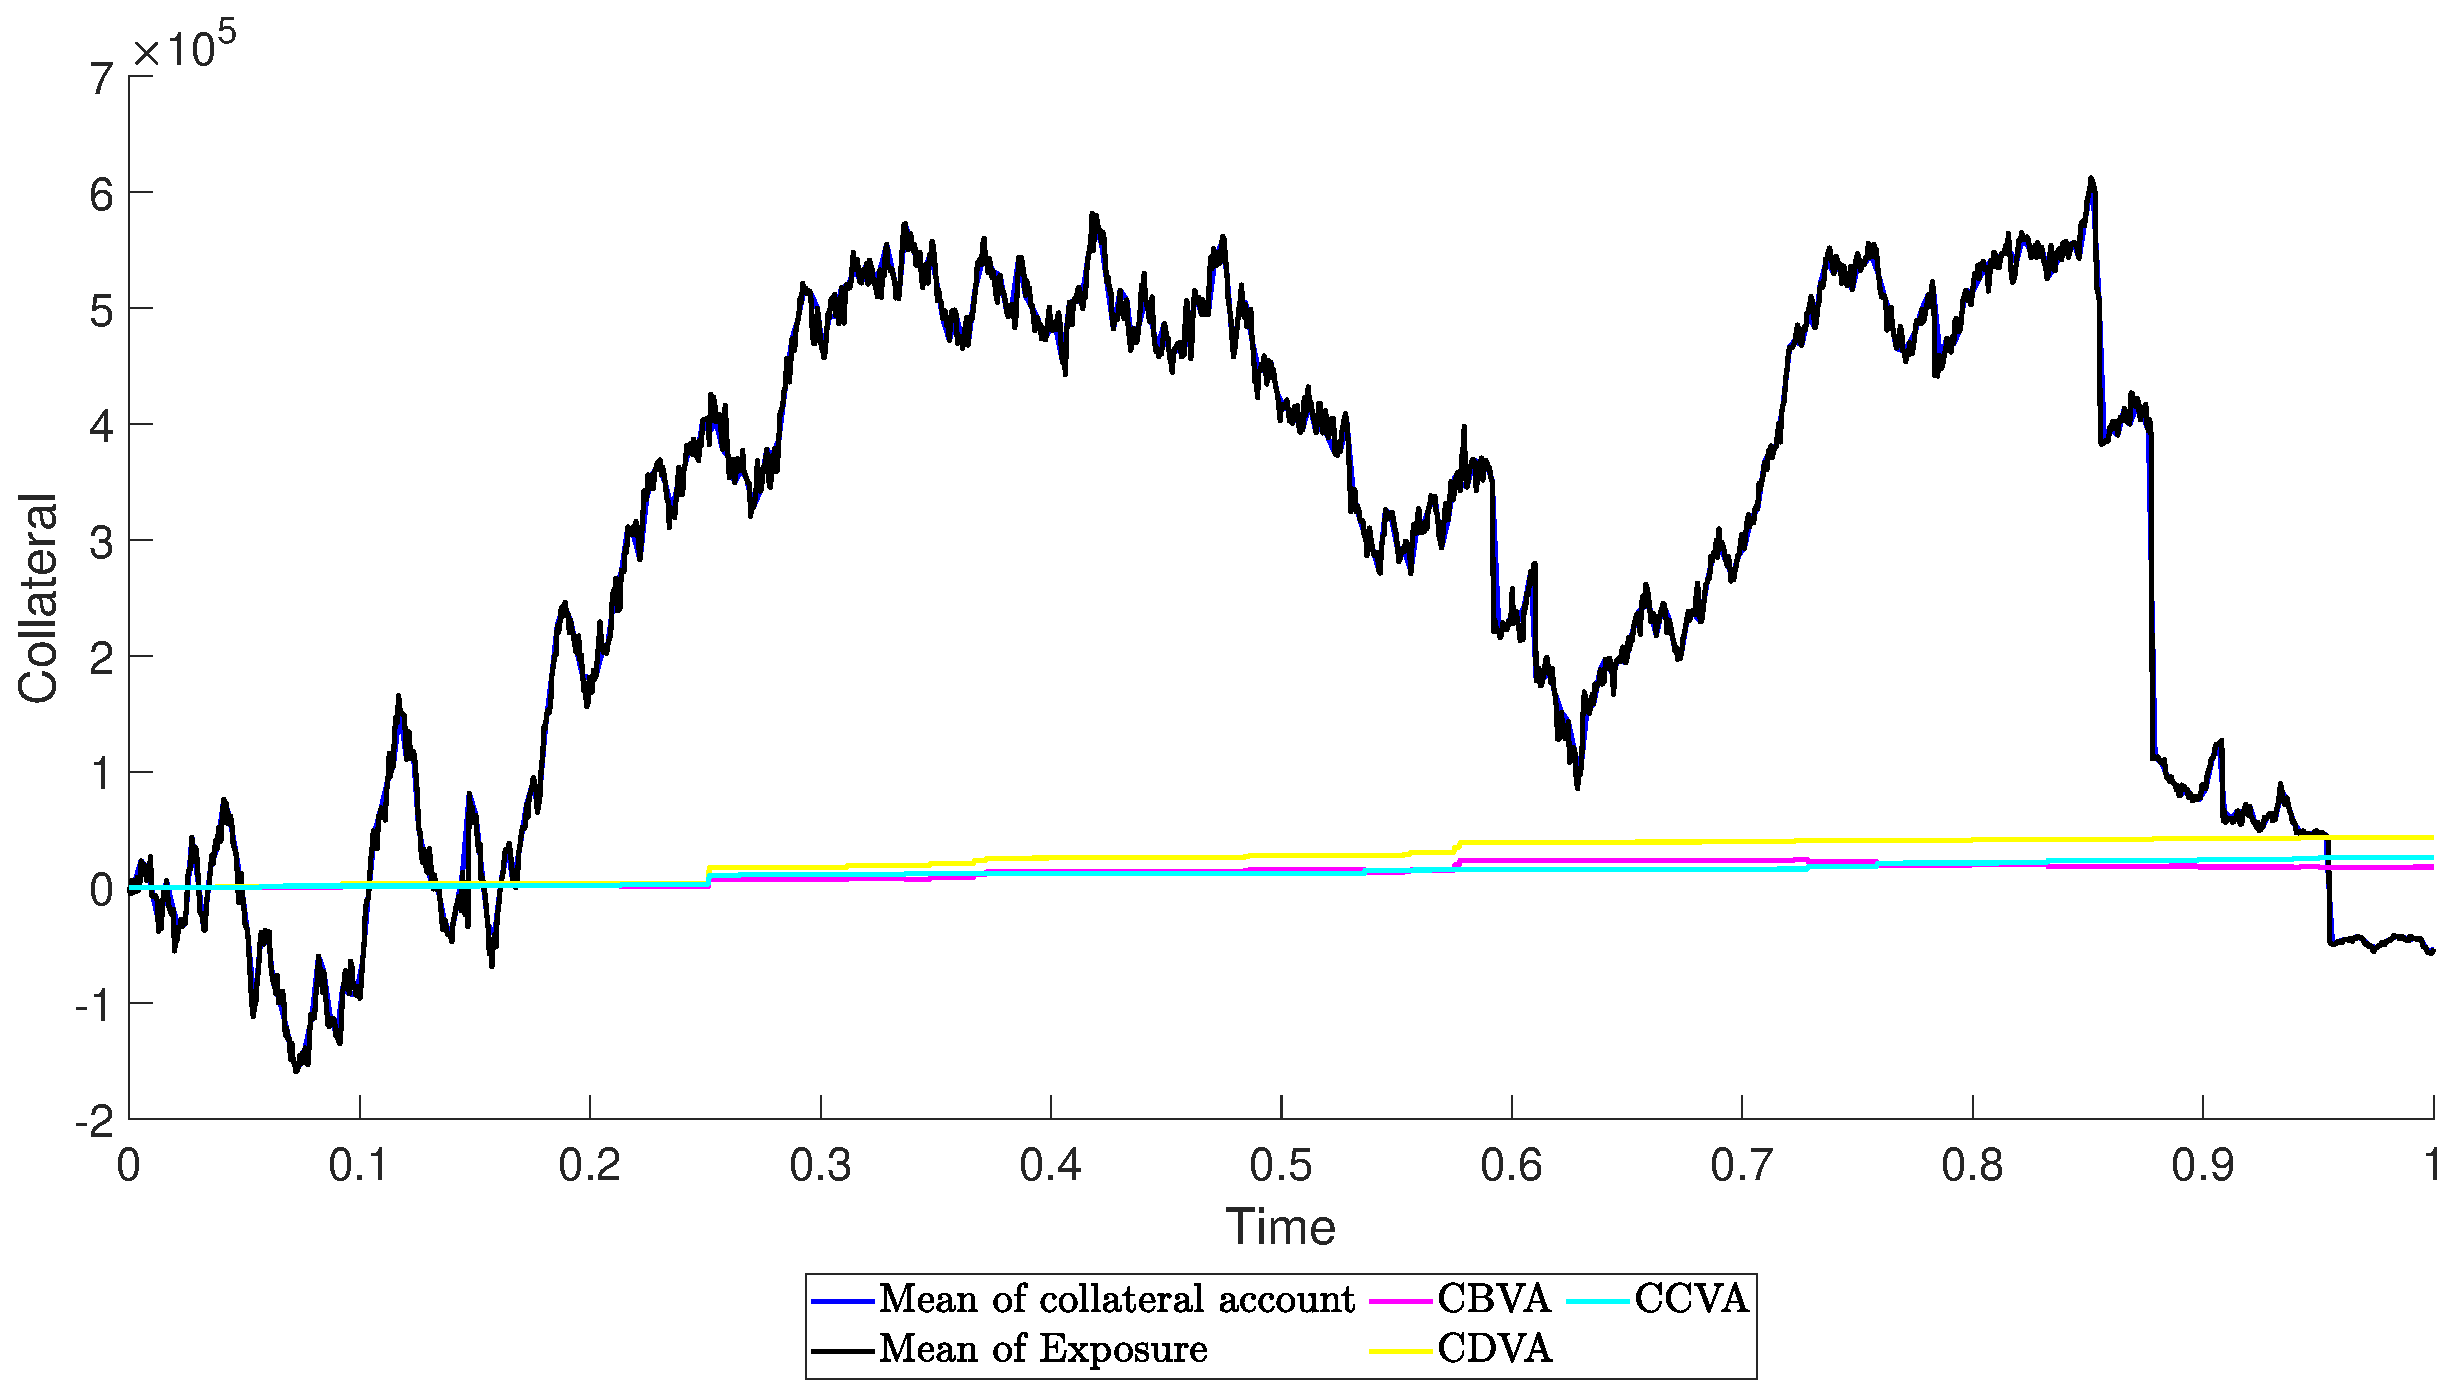
\includegraphics[width=.95\columnwidth]{CVAPC/CVAPC_FOBB_1}
\end{landscape}

\subsection{Pre-default under $\mathbb{P}$}
	\begin{landscape}
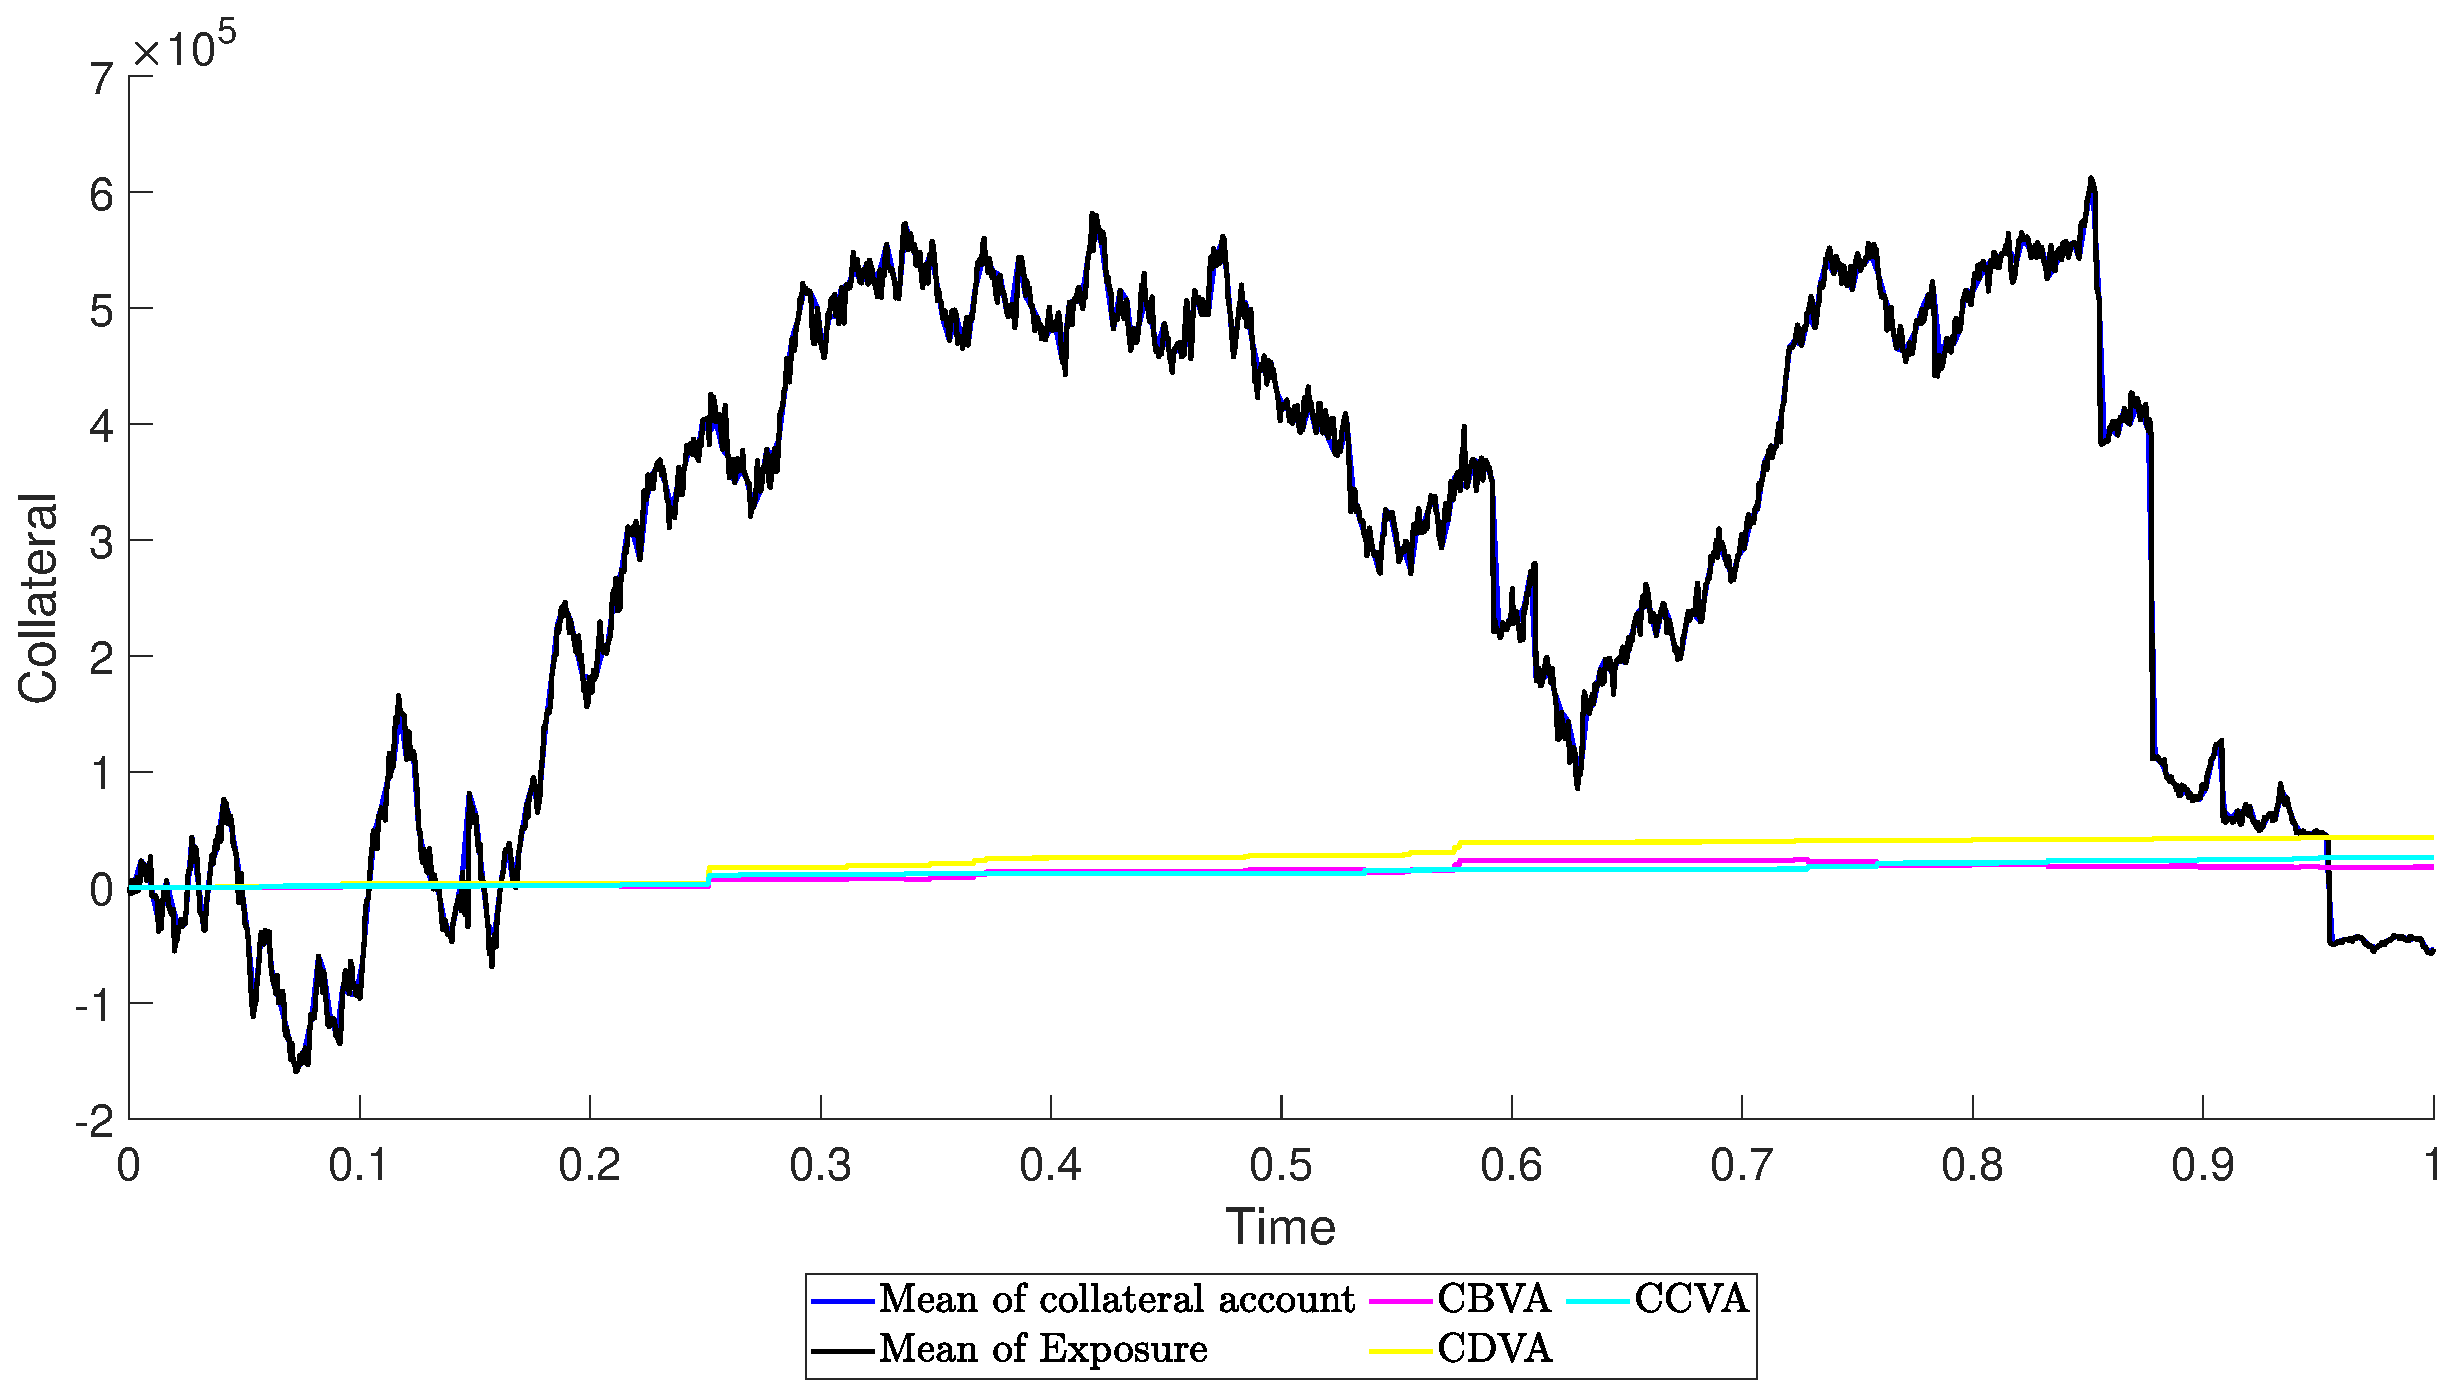
\includegraphics[width=.95\columnwidth]{CVAPC/CVAPC_FOBB_1}
\end{landscape}

\subsection{Collateral and CXVA, $X=B,D,C$}
\subsubsection{Un-collateralized}
	\newcommand{\shortRatePCFOBB}{%
$r=0$%
}%
\newcommand{\shortRatePCFOBBvalue}{%
0%
}%
\newcommand{\LGDIPCFOBB}{%
$\mathrm{LGD}_I=0.6$%
}%
\newcommand{\LGDIPCFOBBvalue}{%
0.6%
}%
\newcommand{\LGDCPCFOBB}{%
$\mathrm{LGD}_C=0.6$%
}%
\newcommand{\LGDCPCFOBBvalue}{%
0.6%
}%
\newcommand{\simulationsPCFOBB}{%
$M=10000$%
}%
\newcommand{\simulationsPCFOBBvalue}{%
10000%
}%
\newcommand{\cbvaPCFOBB}{%
$\mathrm{CBVA}=1.77e+04$%
}%
\newcommand{\cbvaPCFOBBvalue}{%
1.77e+04%
}%
\newcommand{\cdvaPCFOBB}{%
$\mathrm{CDVA}=4.33e+04$%
}%
\newcommand{\cdvaPCFOBBvalue}{%
4.33e+04%
}%
\newcommand{\ccvaPCFOBB}{%
$\mathrm{CCVA}=2.56e+04$%
}%
\newcommand{\ccvaPCFOBBvalue}{%
2.56e+04%
}%
\newcommand{\tresholdsIPCFOBBHeader}{%
F1+ & F1 & F2 & F3 & B & C & D }%
\newcommand{\tresholdsIPCFOBBBody}{%
$ 0$ & $ 0$ & $ 0$ & $ 0$ & $ 0$ & $ 0$ & $ 0$ 
}%
\newcommand{\tresholdsIPCFOBB}{%
\begin{tabular}{|*{7}{c}|}
\hline
F1+ & F1 & F2 & F3 & B & C & D \\$ 0$ & $ 0$ & $ 0$ & $ 0$ & $ 0$ & $ 0$ & $ 0$ 
\\\hline
\end{tabular}
}%
\newcommand{\tresholdsIPCFOBBCaption}{%
\caption{Investor's thresholds}}%
\newcommand{\tresholdsCPCFOBBHeader}{%
F1+ & F1 & F2 & F3 & B & C & D }%
\newcommand{\tresholdsCPCFOBBBody}{%
$ 0$ & $ 0$ & $ 0$ & $ 0$ & $ 0$ & $ 0$ & $ 0$ 
}%
\newcommand{\tresholdsCPCFOBB}{%
\begin{tabular}{|*{7}{c}|}
\hline
F1+ & F1 & F2 & F3 & B & C & D \\$ 0$ & $ 0$ & $ 0$ & $ 0$ & $ 0$ & $ 0$ & $ 0$ 
\\\hline
\end{tabular}
}%
\newcommand{\tresholdsCPCFOBBCaption}{%
\caption{Counterparty's thresholds}}%

	\shortRateUCFOBB\hfill\\
	\LGDIUCFOBB\hfill\\
	\LGDCUCFOBB\hfill\\
	\simulationsUCFOBB\hfill\\
	\cbvaUCFOBB\hfill\\
	\cdvaUCFOBB\hfill\\
	\ccvaUCFOBB\hfill\\
\begin{table}[h!]
	\tresholdsIUCFOBB%
\centering
\tresholdsIUCFOBBCaption
\label{tab:thresholds8}
\end{table}
\begin{table}[h!]
	\tresholdsCUCFOBB%
\centering
\tresholdsCUCFOBBCaption
\label{tab:thresholds9}
\end{table}
	\begin{landscape}
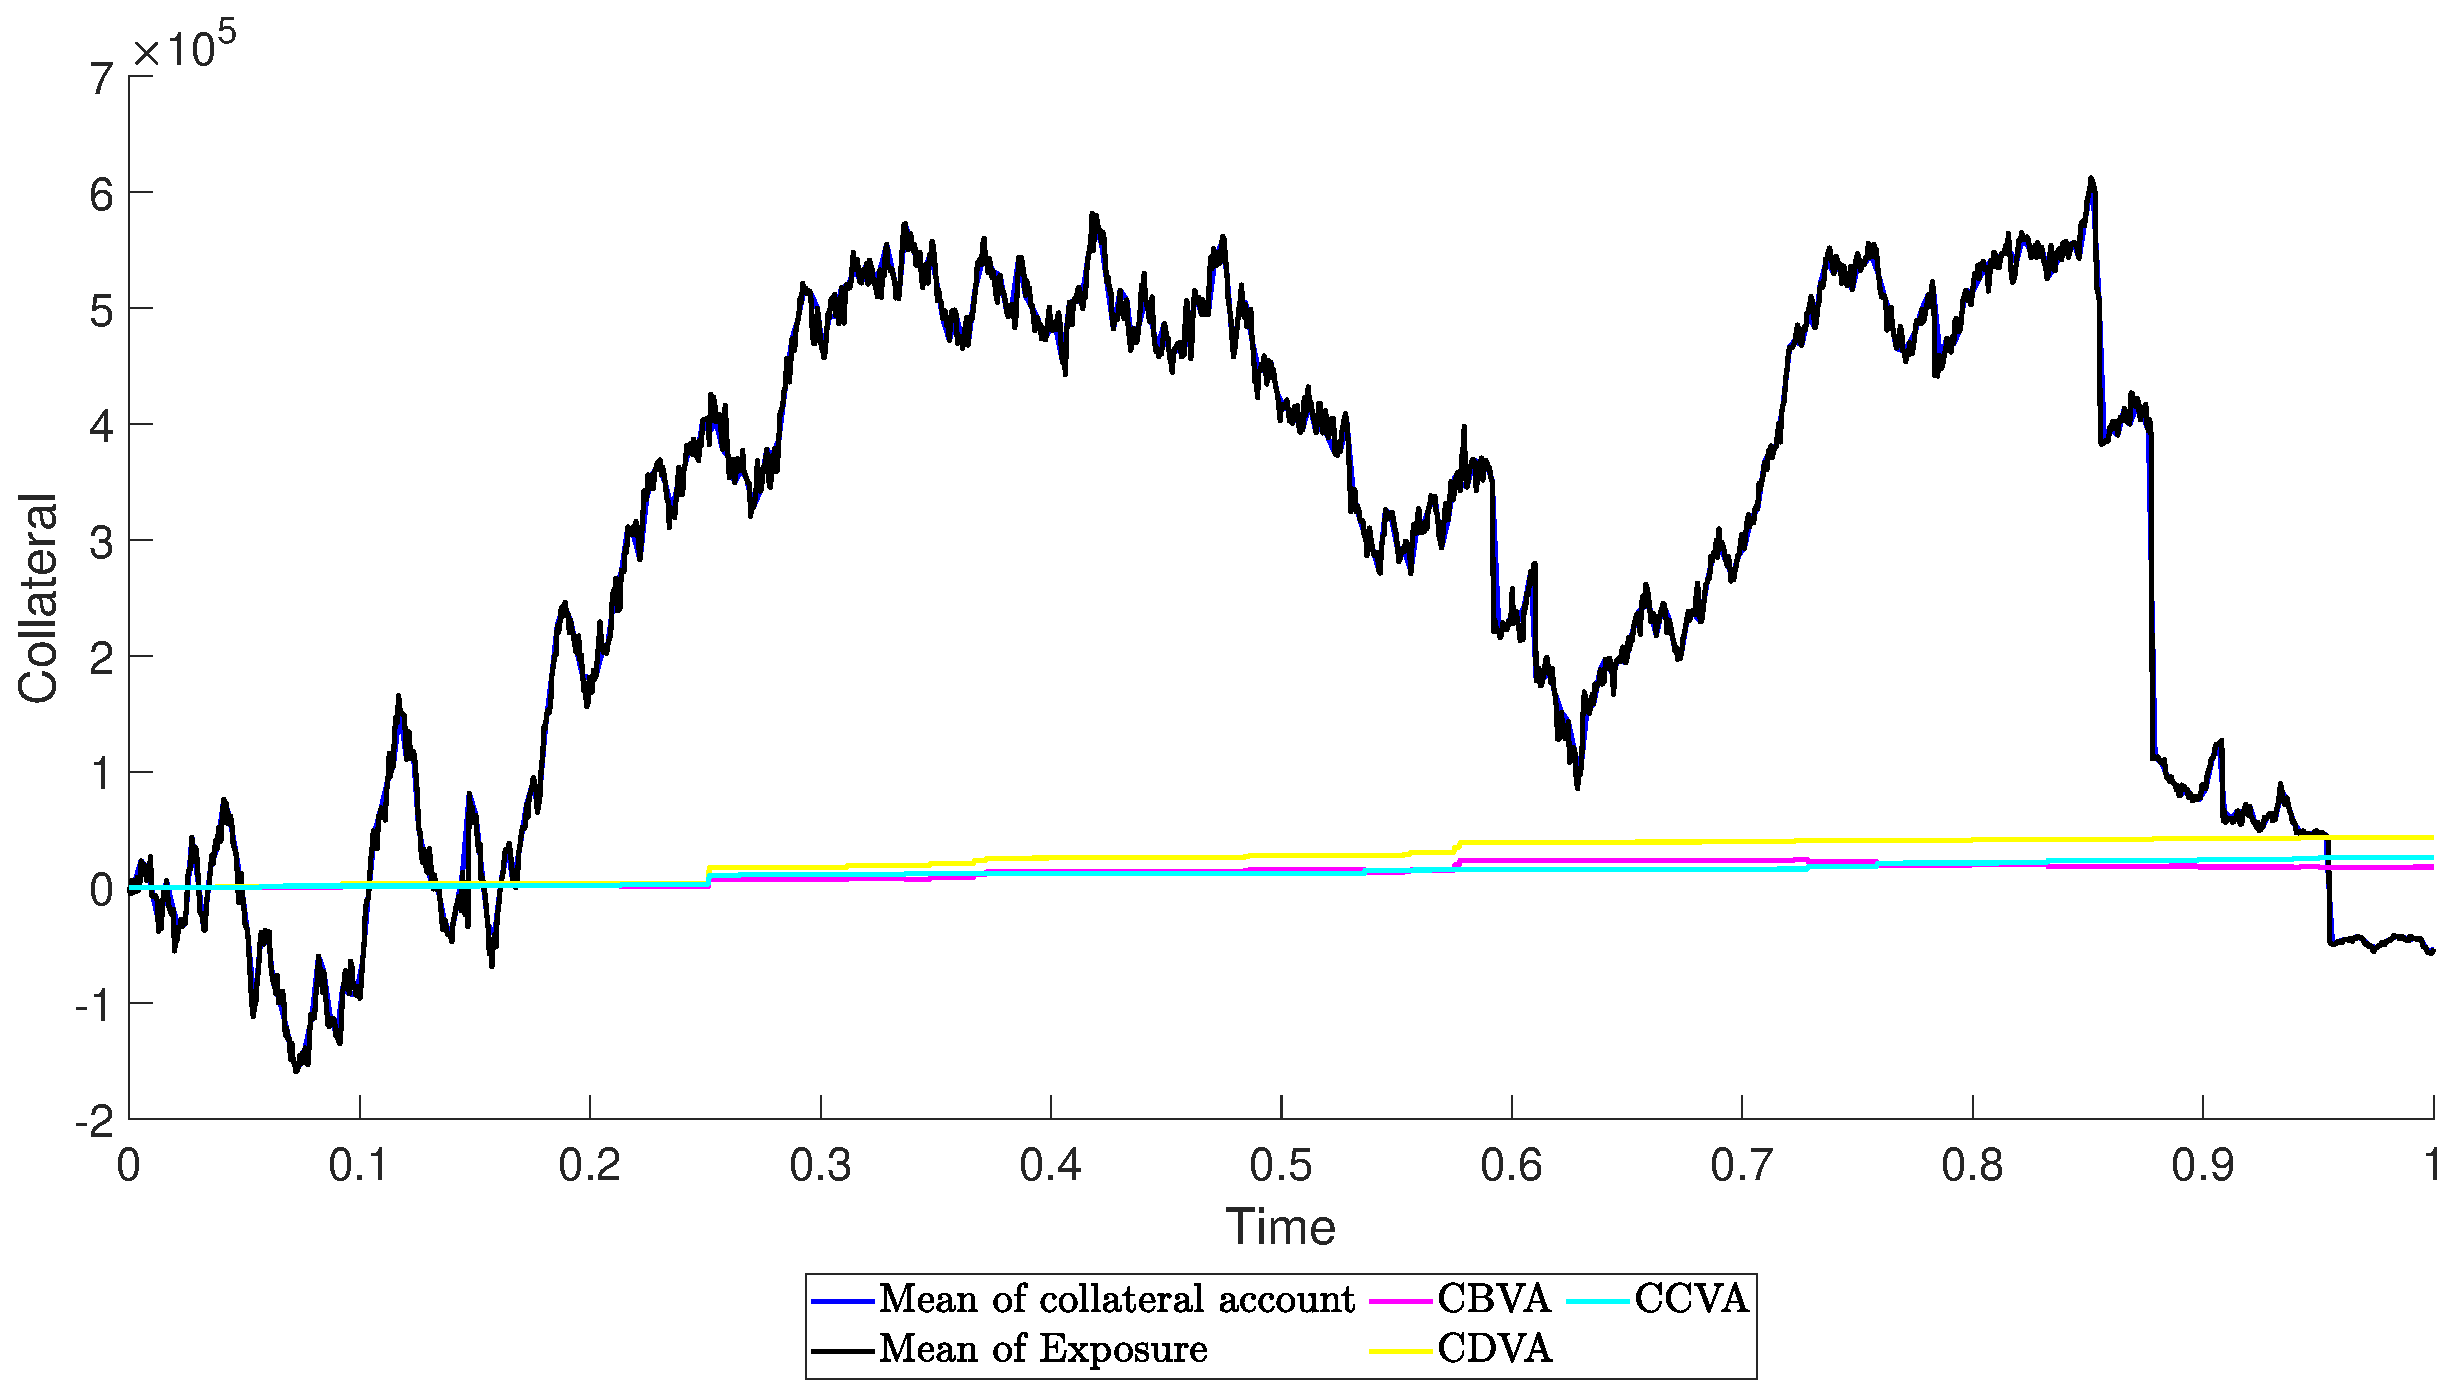
\includegraphics[width=.95\columnwidth]{CVAPC/CVAPC_FOBB_1}
\end{landscape}

\paragraph*{CVA}
	\begin{landscape}
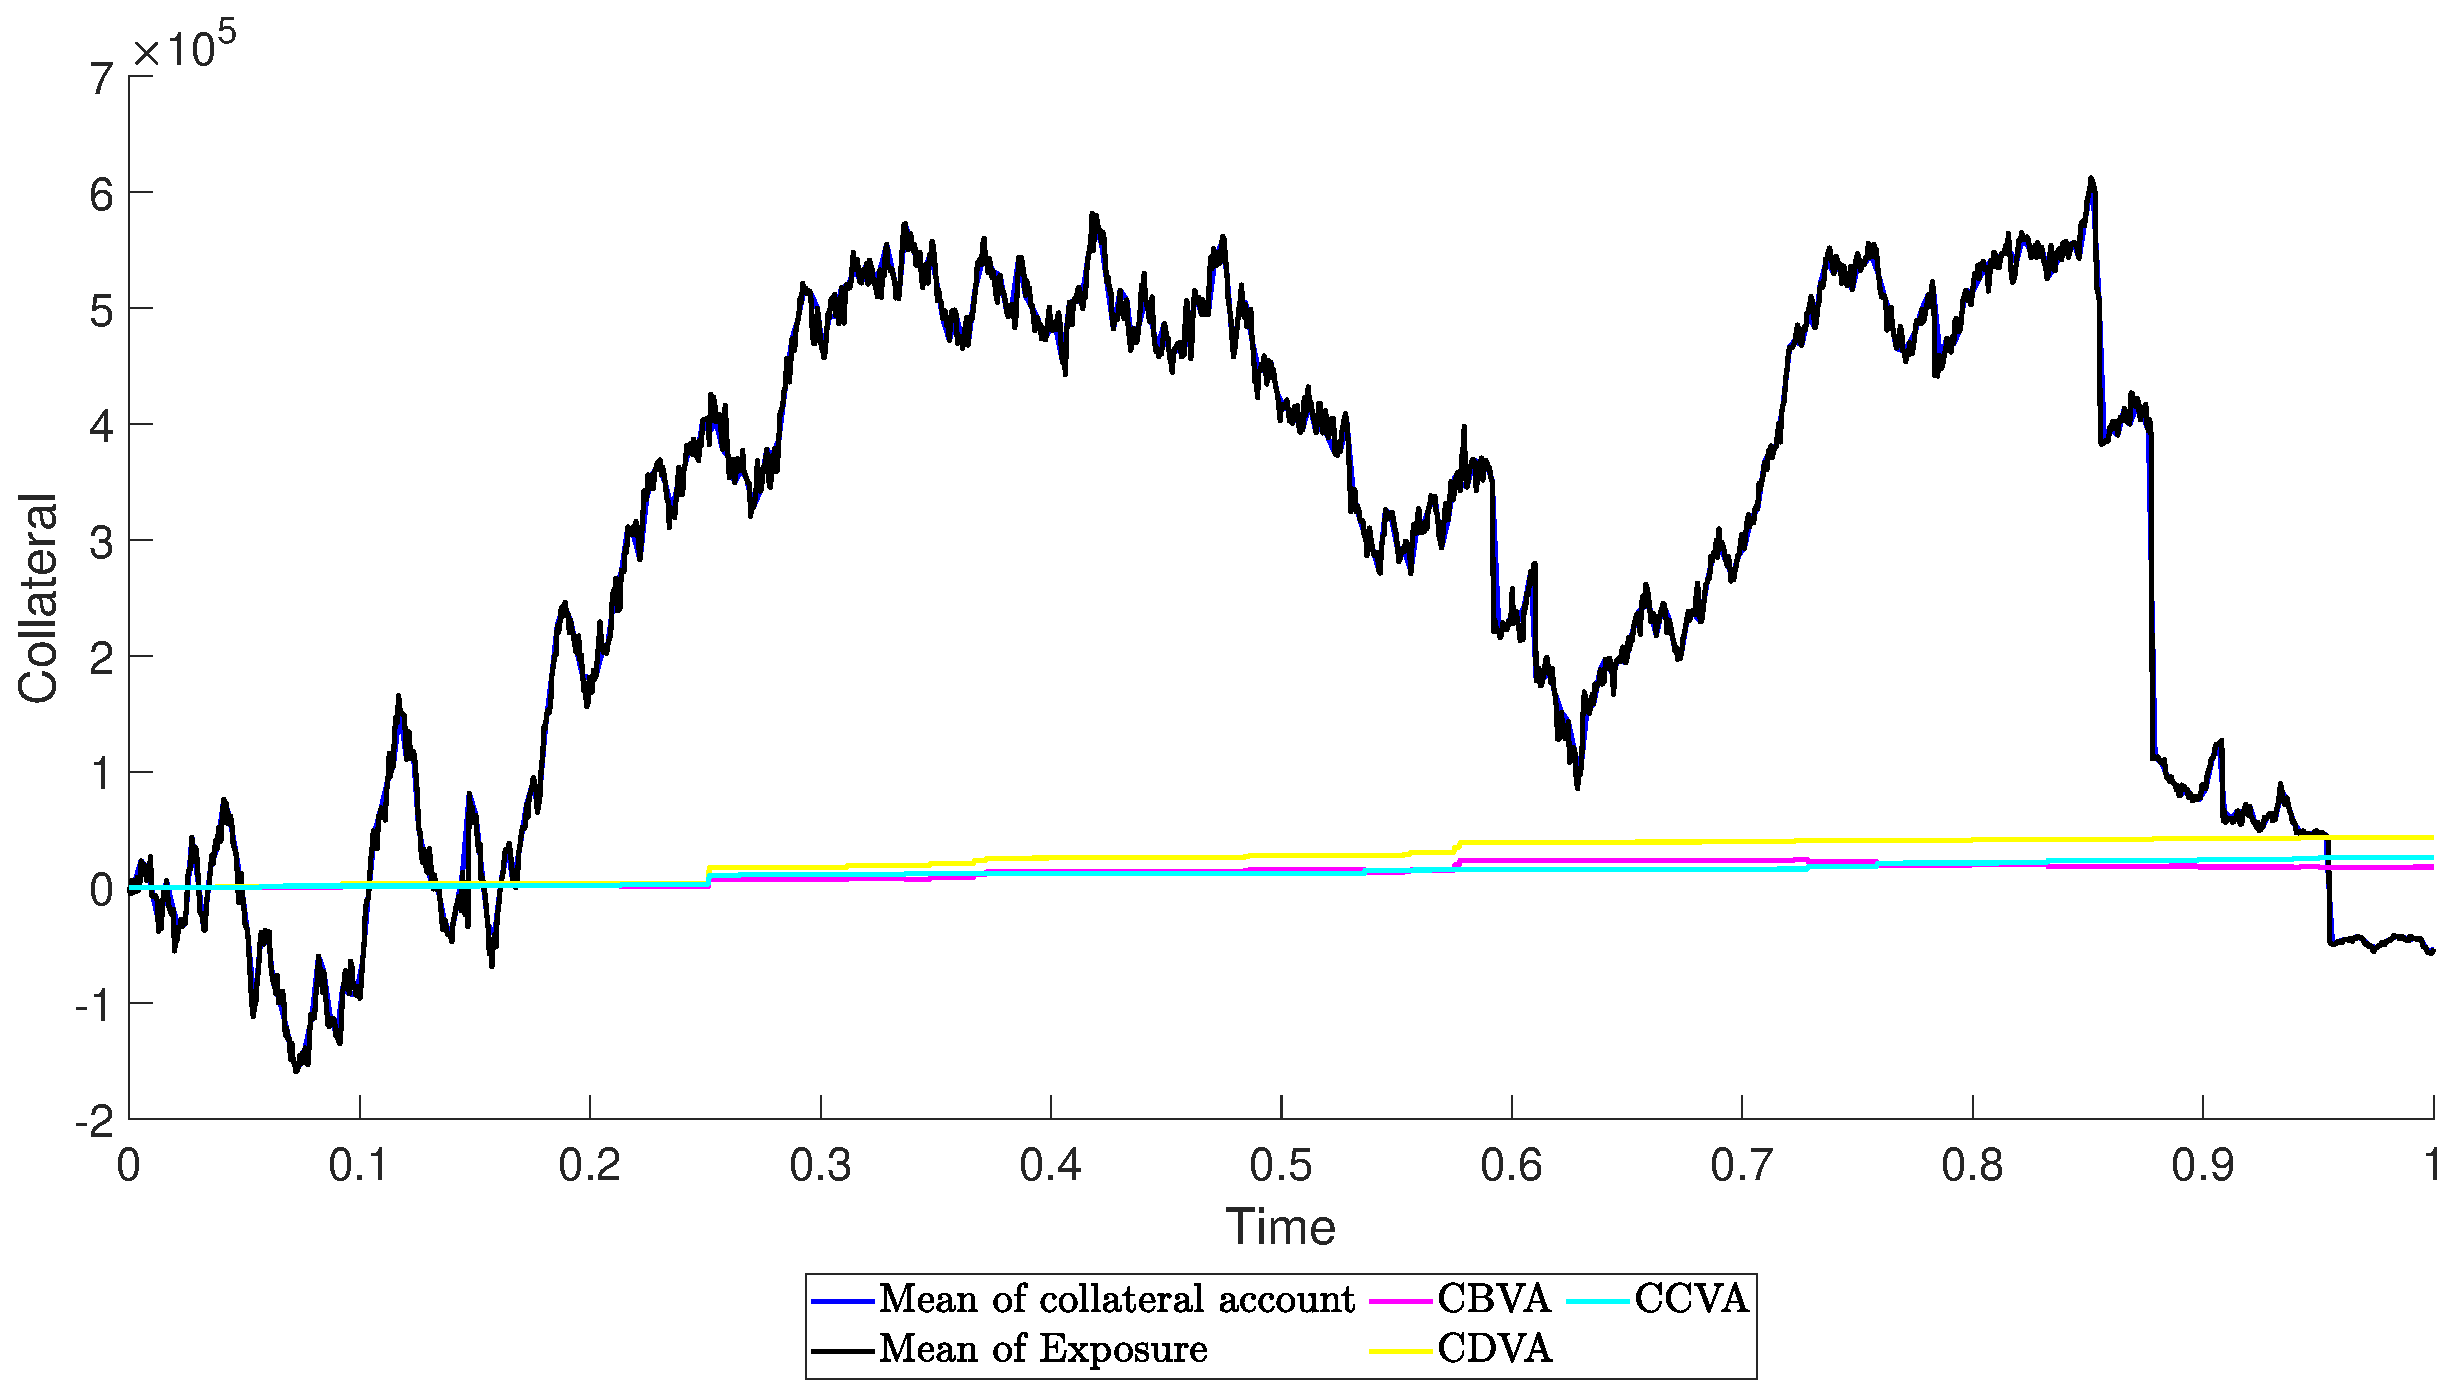
\includegraphics[width=.95\columnwidth]{CVAPC/CVAPC_FOBB_1}
\end{landscape}

\subsubsection{Collateralized with rating triggers}
	\newcommand{\shortRatePCFOBB}{%
$r=0$%
}%
\newcommand{\shortRatePCFOBBvalue}{%
0%
}%
\newcommand{\LGDIPCFOBB}{%
$\mathrm{LGD}_I=0.6$%
}%
\newcommand{\LGDIPCFOBBvalue}{%
0.6%
}%
\newcommand{\LGDCPCFOBB}{%
$\mathrm{LGD}_C=0.6$%
}%
\newcommand{\LGDCPCFOBBvalue}{%
0.6%
}%
\newcommand{\simulationsPCFOBB}{%
$M=10000$%
}%
\newcommand{\simulationsPCFOBBvalue}{%
10000%
}%
\newcommand{\cbvaPCFOBB}{%
$\mathrm{CBVA}=1.77e+04$%
}%
\newcommand{\cbvaPCFOBBvalue}{%
1.77e+04%
}%
\newcommand{\cdvaPCFOBB}{%
$\mathrm{CDVA}=4.33e+04$%
}%
\newcommand{\cdvaPCFOBBvalue}{%
4.33e+04%
}%
\newcommand{\ccvaPCFOBB}{%
$\mathrm{CCVA}=2.56e+04$%
}%
\newcommand{\ccvaPCFOBBvalue}{%
2.56e+04%
}%
\newcommand{\tresholdsIPCFOBBHeader}{%
F1+ & F1 & F2 & F3 & B & C & D }%
\newcommand{\tresholdsIPCFOBBBody}{%
$ 0$ & $ 0$ & $ 0$ & $ 0$ & $ 0$ & $ 0$ & $ 0$ 
}%
\newcommand{\tresholdsIPCFOBB}{%
\begin{tabular}{|*{7}{c}|}
\hline
F1+ & F1 & F2 & F3 & B & C & D \\$ 0$ & $ 0$ & $ 0$ & $ 0$ & $ 0$ & $ 0$ & $ 0$ 
\\\hline
\end{tabular}
}%
\newcommand{\tresholdsIPCFOBBCaption}{%
\caption{Investor's thresholds}}%
\newcommand{\tresholdsCPCFOBBHeader}{%
F1+ & F1 & F2 & F3 & B & C & D }%
\newcommand{\tresholdsCPCFOBBBody}{%
$ 0$ & $ 0$ & $ 0$ & $ 0$ & $ 0$ & $ 0$ & $ 0$ 
}%
\newcommand{\tresholdsCPCFOBB}{%
\begin{tabular}{|*{7}{c}|}
\hline
F1+ & F1 & F2 & F3 & B & C & D \\$ 0$ & $ 0$ & $ 0$ & $ 0$ & $ 0$ & $ 0$ & $ 0$ 
\\\hline
\end{tabular}
}%
\newcommand{\tresholdsCPCFOBBCaption}{%
\caption{Counterparty's thresholds}}%

	\shortRateRTFOBB\hfill\\
	\LGDIRTFOBB\hfill\\
	\LGDCRTFOBB\hfill\\
	\simulationsRTFOBB\hfill\\
	\cbvaRTFOBB\hfill\\
	\cdvaRTFOBB\hfill\\
	\ccvaRTFOBB\hfill\\
\begin{table}[h!]
	\tresholdsIRTFOBB%
\centering
\tresholdsIRTFOBBCaption
\label{tab:thresholds8}
\end{table}
\begin{table}[h!]
	\tresholdsCRTFOBB%
\centering
\tresholdsCRTFOBBCaption
\label{tab:thresholds9}
\end{table}
	\begin{landscape}
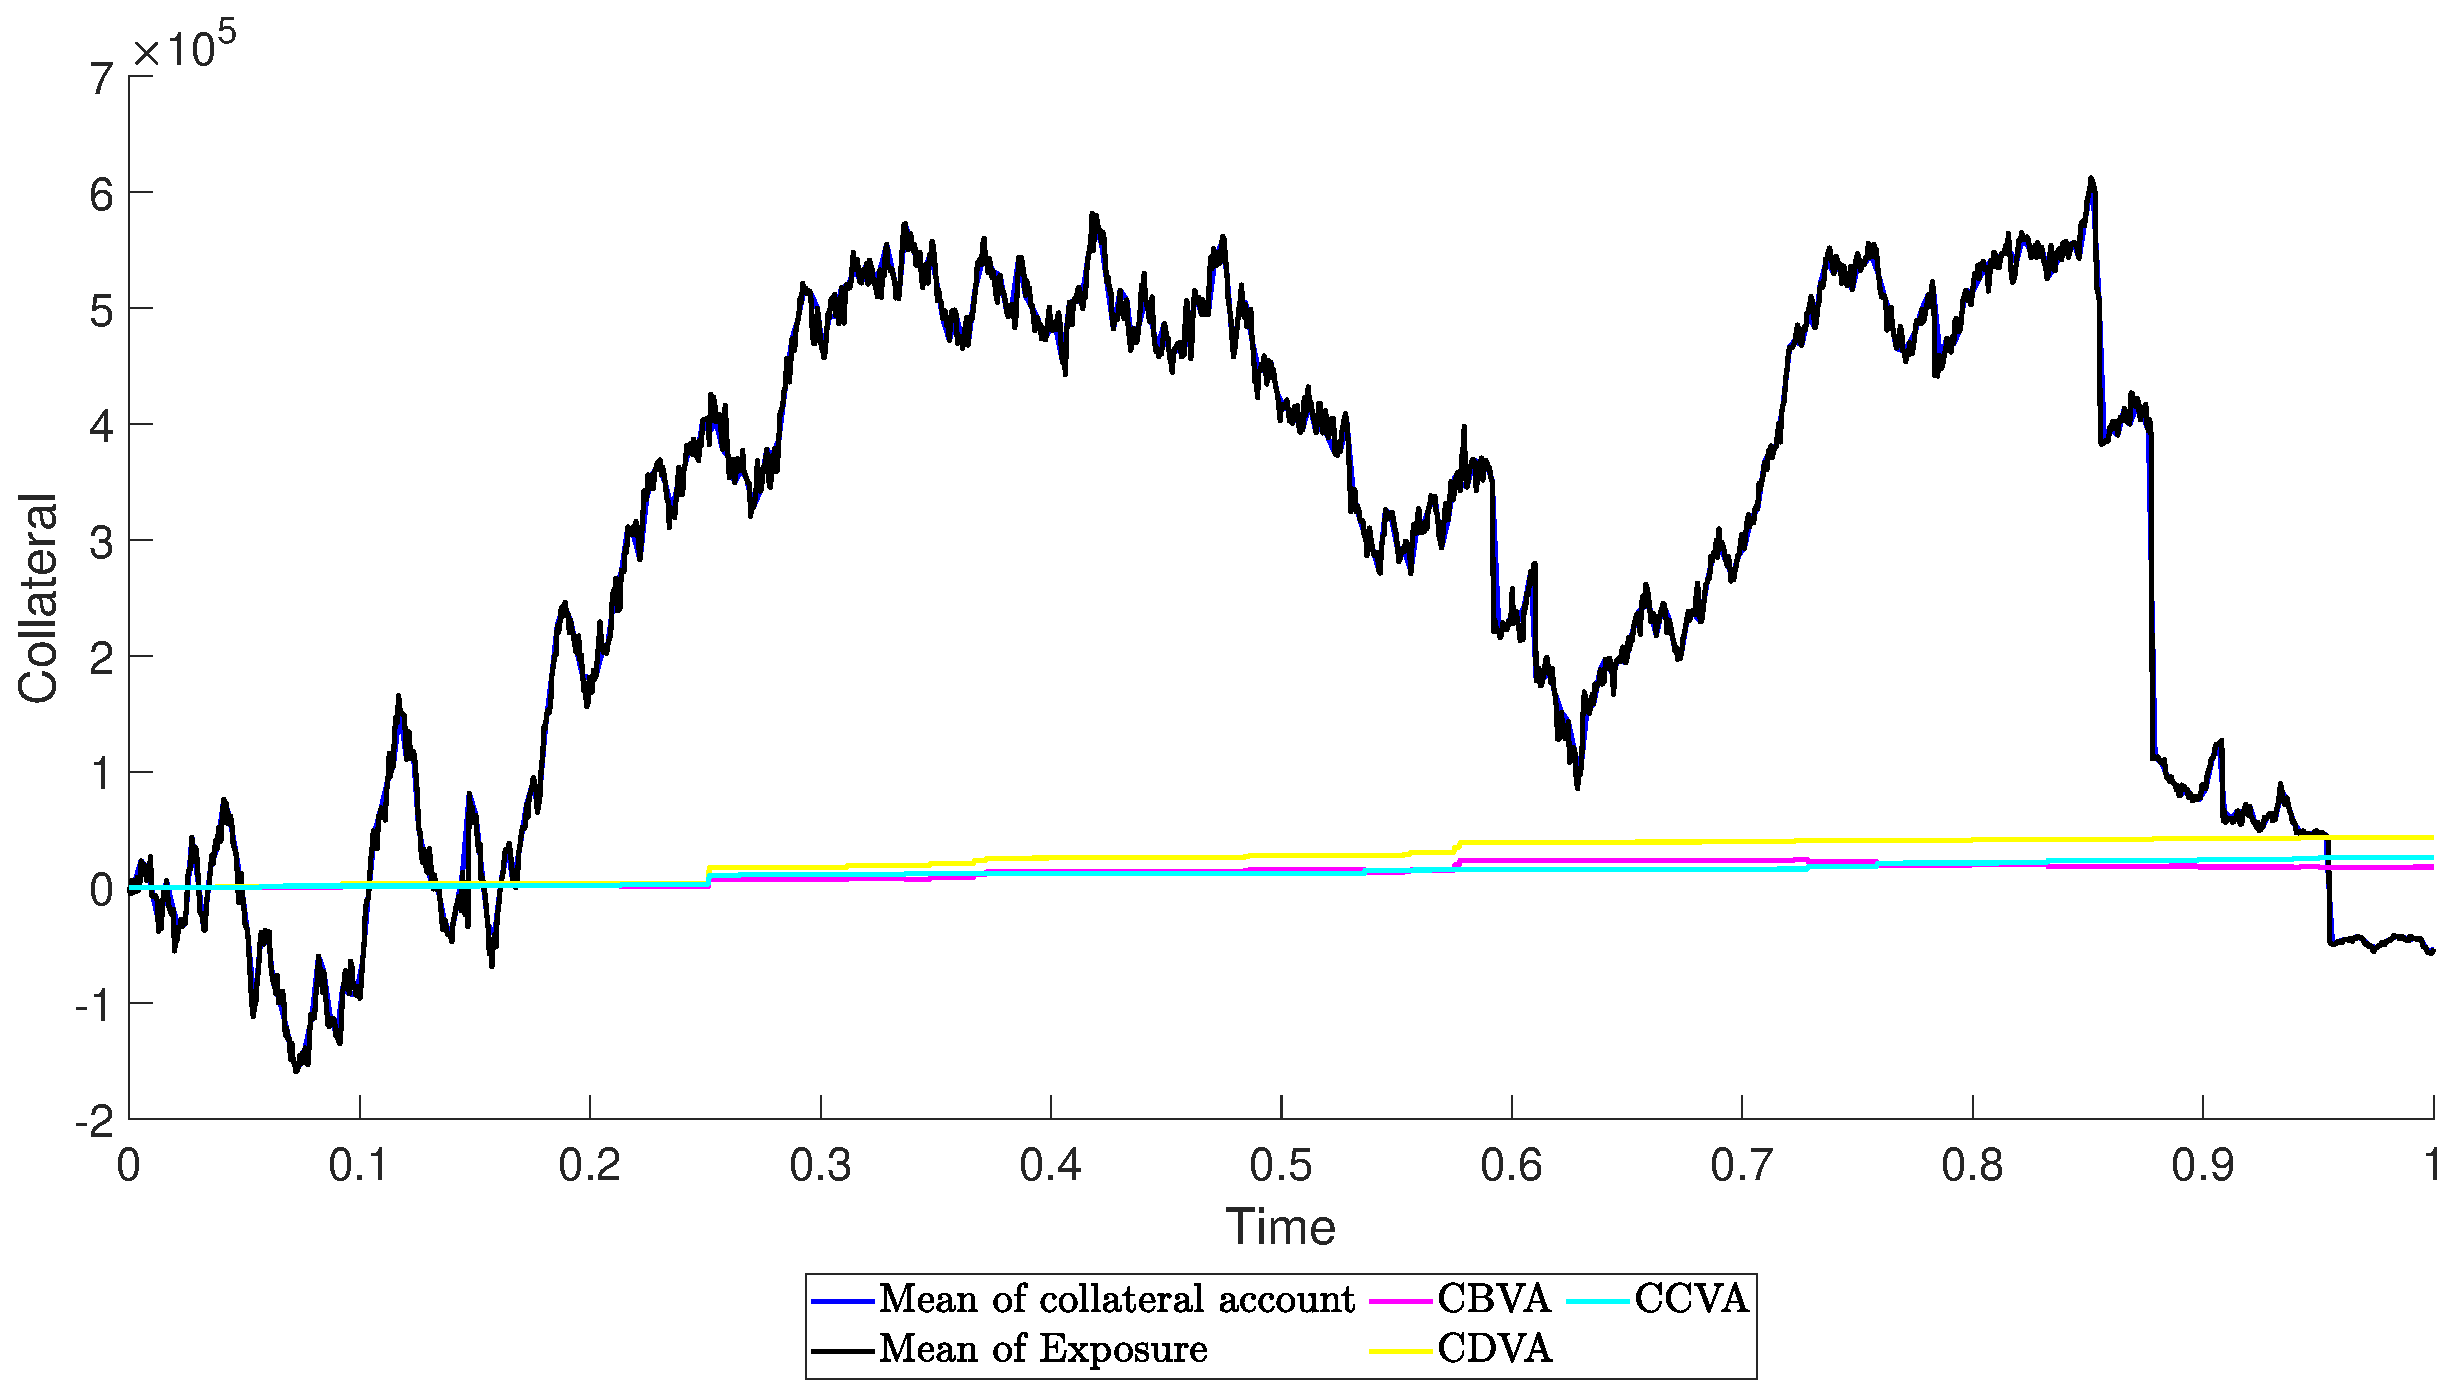
\includegraphics[width=.95\columnwidth]{CVAPC/CVAPC_FOBB_1}
\end{landscape}

\paragraph*{CVA}
	\begin{landscape}
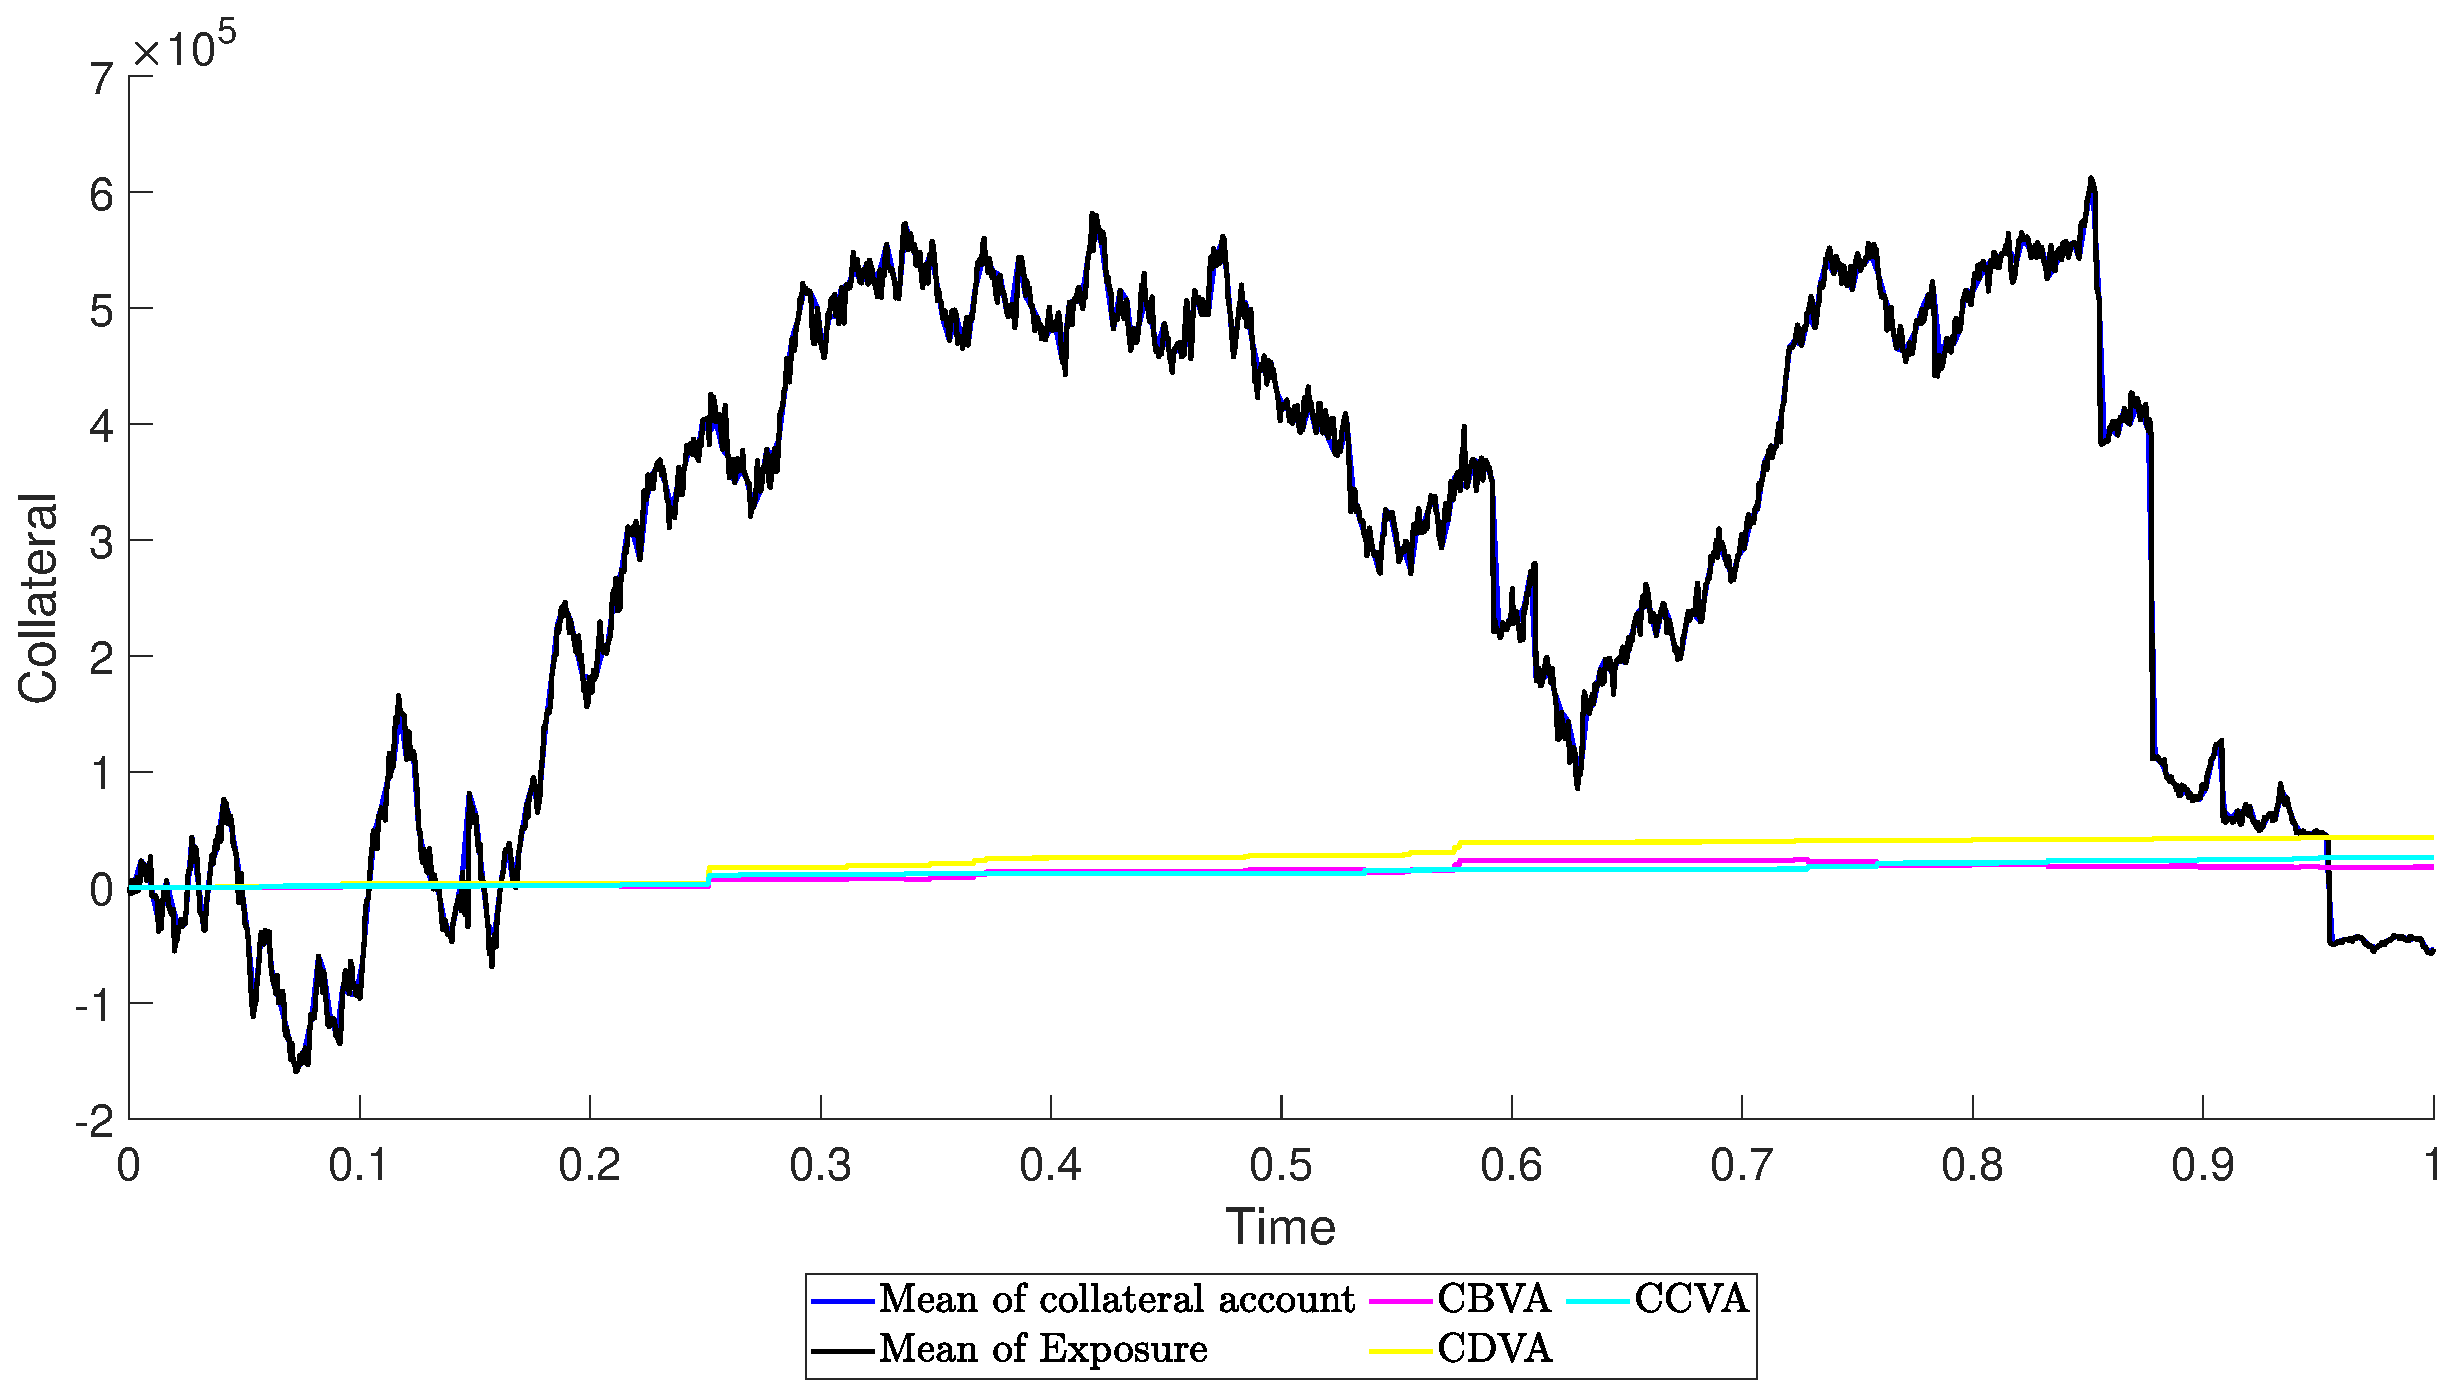
\includegraphics[width=.95\columnwidth]{CVAPC/CVAPC_FOBB_1}
\end{landscape}

\subsubsection{Perfectly collateralized}
	\newcommand{\shortRatePCFOBB}{%
$r=0$%
}%
\newcommand{\shortRatePCFOBBvalue}{%
0%
}%
\newcommand{\LGDIPCFOBB}{%
$\mathrm{LGD}_I=0.6$%
}%
\newcommand{\LGDIPCFOBBvalue}{%
0.6%
}%
\newcommand{\LGDCPCFOBB}{%
$\mathrm{LGD}_C=0.6$%
}%
\newcommand{\LGDCPCFOBBvalue}{%
0.6%
}%
\newcommand{\simulationsPCFOBB}{%
$M=10000$%
}%
\newcommand{\simulationsPCFOBBvalue}{%
10000%
}%
\newcommand{\cbvaPCFOBB}{%
$\mathrm{CBVA}=1.77e+04$%
}%
\newcommand{\cbvaPCFOBBvalue}{%
1.77e+04%
}%
\newcommand{\cdvaPCFOBB}{%
$\mathrm{CDVA}=4.33e+04$%
}%
\newcommand{\cdvaPCFOBBvalue}{%
4.33e+04%
}%
\newcommand{\ccvaPCFOBB}{%
$\mathrm{CCVA}=2.56e+04$%
}%
\newcommand{\ccvaPCFOBBvalue}{%
2.56e+04%
}%
\newcommand{\tresholdsIPCFOBBHeader}{%
F1+ & F1 & F2 & F3 & B & C & D }%
\newcommand{\tresholdsIPCFOBBBody}{%
$ 0$ & $ 0$ & $ 0$ & $ 0$ & $ 0$ & $ 0$ & $ 0$ 
}%
\newcommand{\tresholdsIPCFOBB}{%
\begin{tabular}{|*{7}{c}|}
\hline
F1+ & F1 & F2 & F3 & B & C & D \\$ 0$ & $ 0$ & $ 0$ & $ 0$ & $ 0$ & $ 0$ & $ 0$ 
\\\hline
\end{tabular}
}%
\newcommand{\tresholdsIPCFOBBCaption}{%
\caption{Investor's thresholds}}%
\newcommand{\tresholdsCPCFOBBHeader}{%
F1+ & F1 & F2 & F3 & B & C & D }%
\newcommand{\tresholdsCPCFOBBBody}{%
$ 0$ & $ 0$ & $ 0$ & $ 0$ & $ 0$ & $ 0$ & $ 0$ 
}%
\newcommand{\tresholdsCPCFOBB}{%
\begin{tabular}{|*{7}{c}|}
\hline
F1+ & F1 & F2 & F3 & B & C & D \\$ 0$ & $ 0$ & $ 0$ & $ 0$ & $ 0$ & $ 0$ & $ 0$ 
\\\hline
\end{tabular}
}%
\newcommand{\tresholdsCPCFOBBCaption}{%
\caption{Counterparty's thresholds}}%

	\shortRatePCFOBB\hfill\\
	\LGDIPCFOBB\hfill\\
	\LGDCPCFOBB\hfill\\
	\simulationsPCFOBB\hfill\\
	\cbvaPCFOBB\hfill\\
	\cdvaPCFOBB\hfill\\
	\ccvaPCFOBB\hfill\\
\begin{table}[h!]
	\tresholdsIPCFOBB%
\centering
\tresholdsIPCFOBBCaption
\label{tab:thresholds8}
\end{table}
\begin{table}[h!]
	\tresholdsCPCFOBB%
\centering
\tresholdsCPCFOBBCaption
\label{tab:thresholds9}
\end{table}
	\begin{landscape}
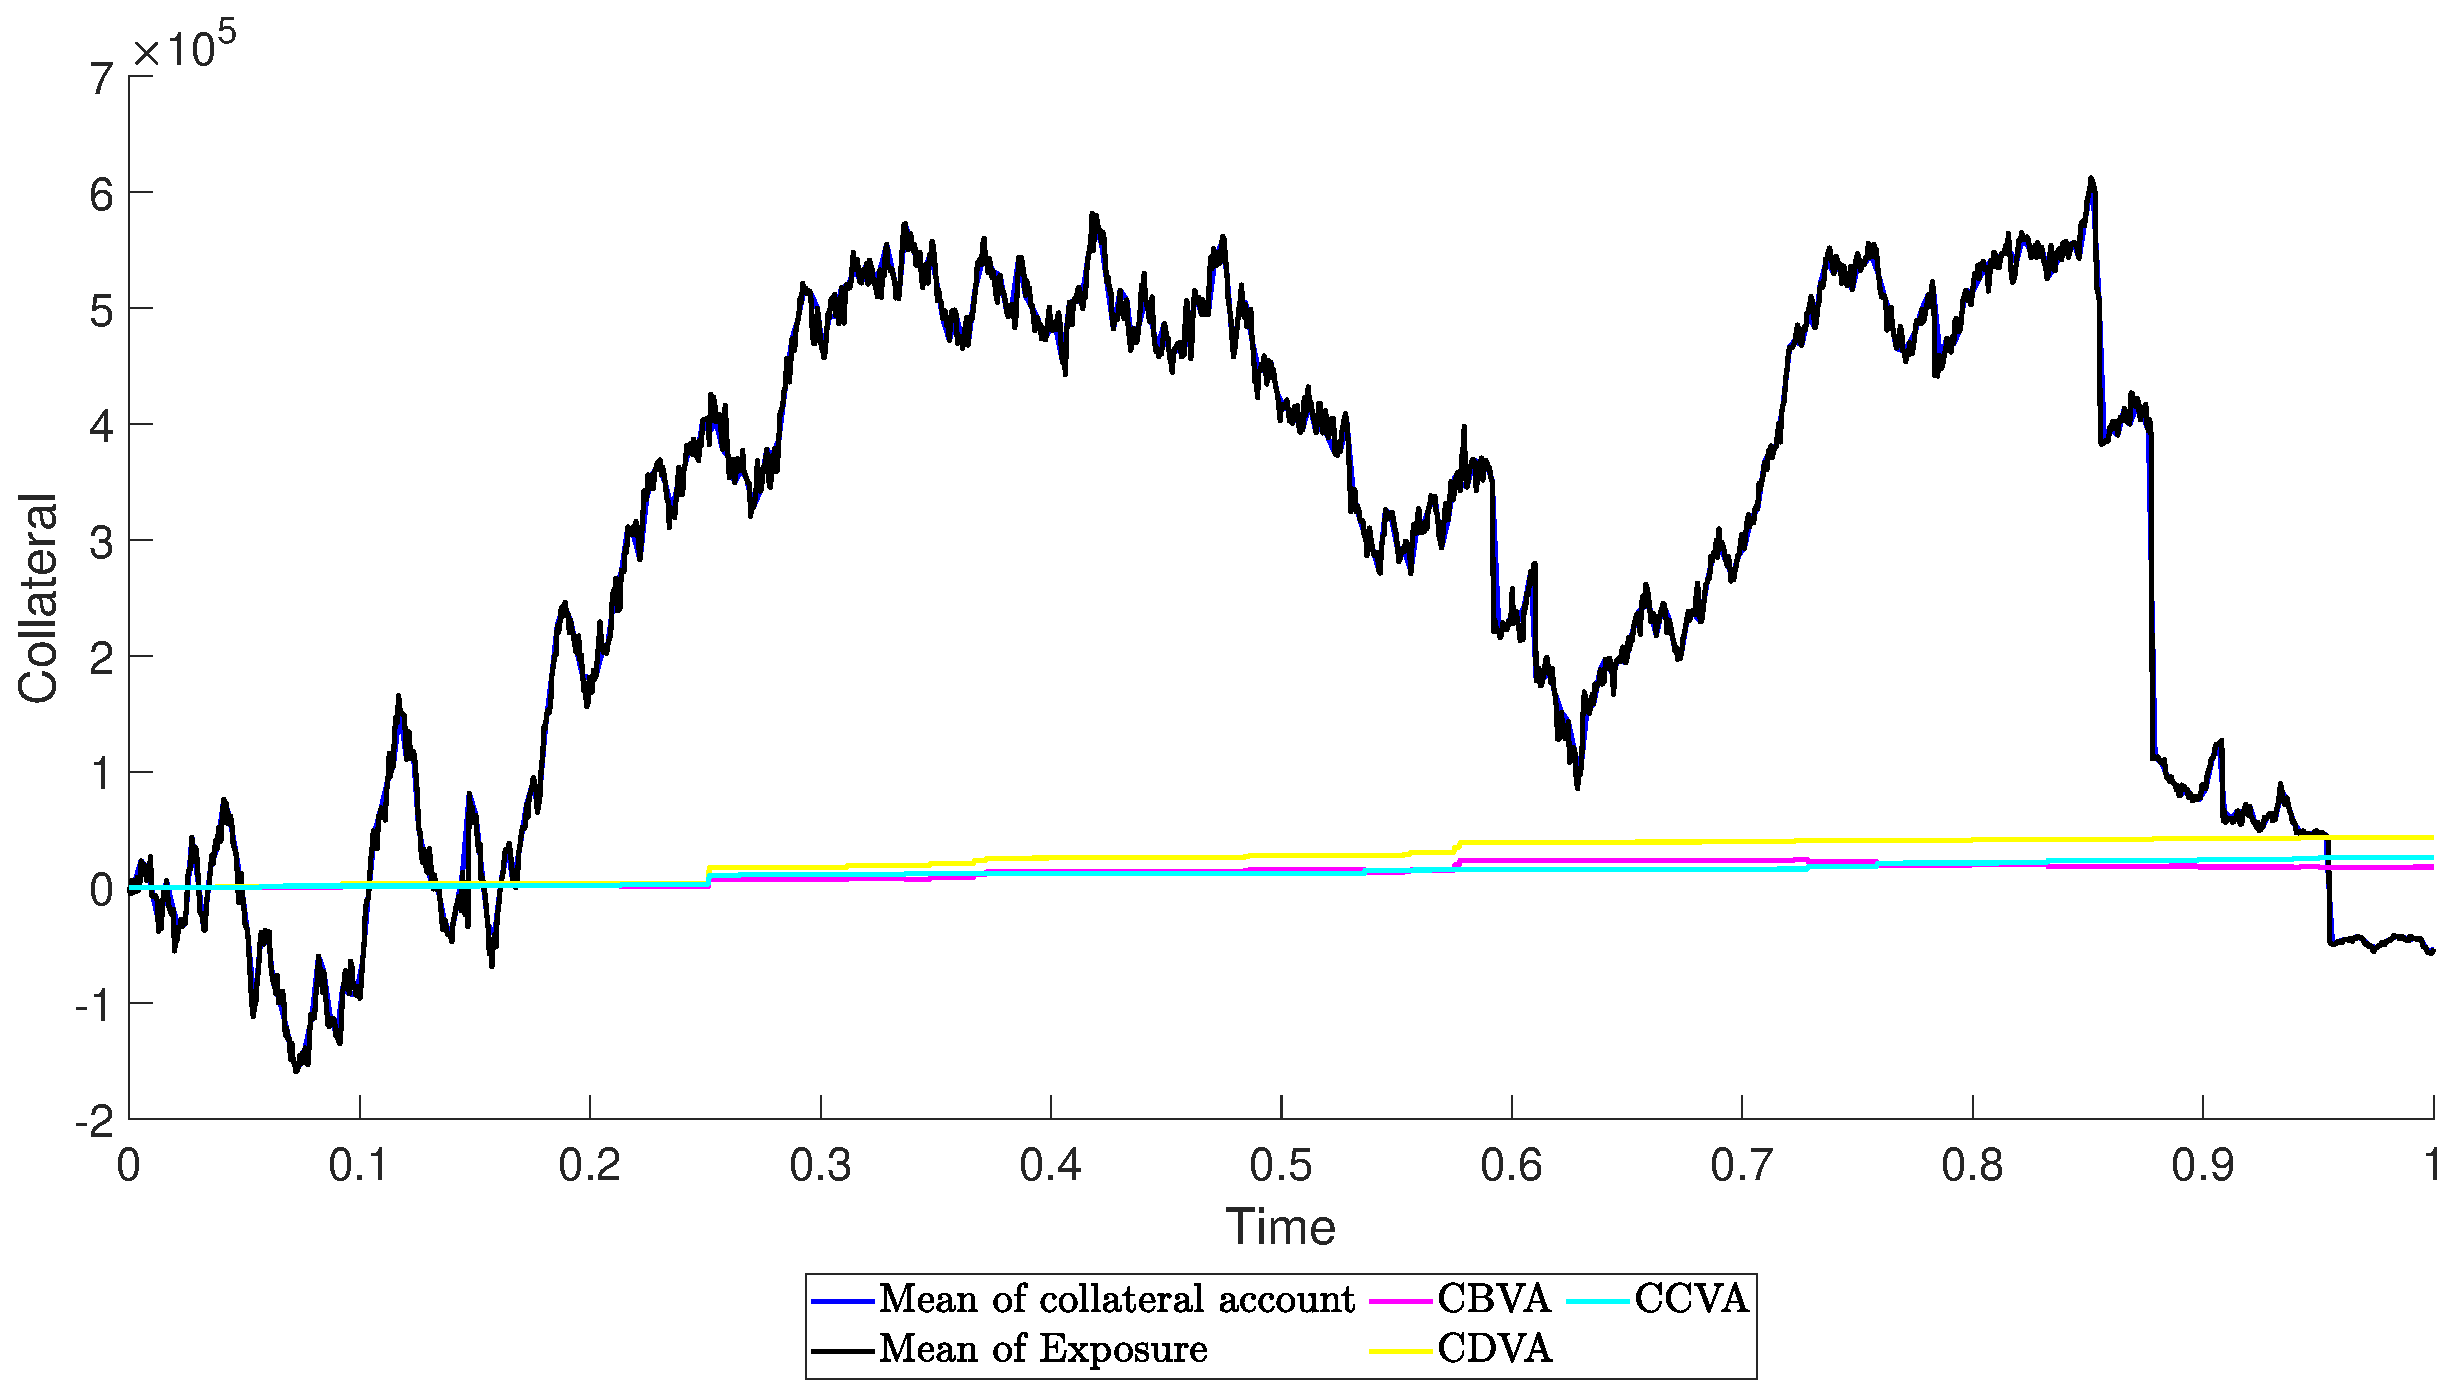
\includegraphics[width=.95\columnwidth]{CVAPC/CVAPC_FOBB_1}
\end{landscape}

\paragraph*{CVA}
	\begin{landscape}
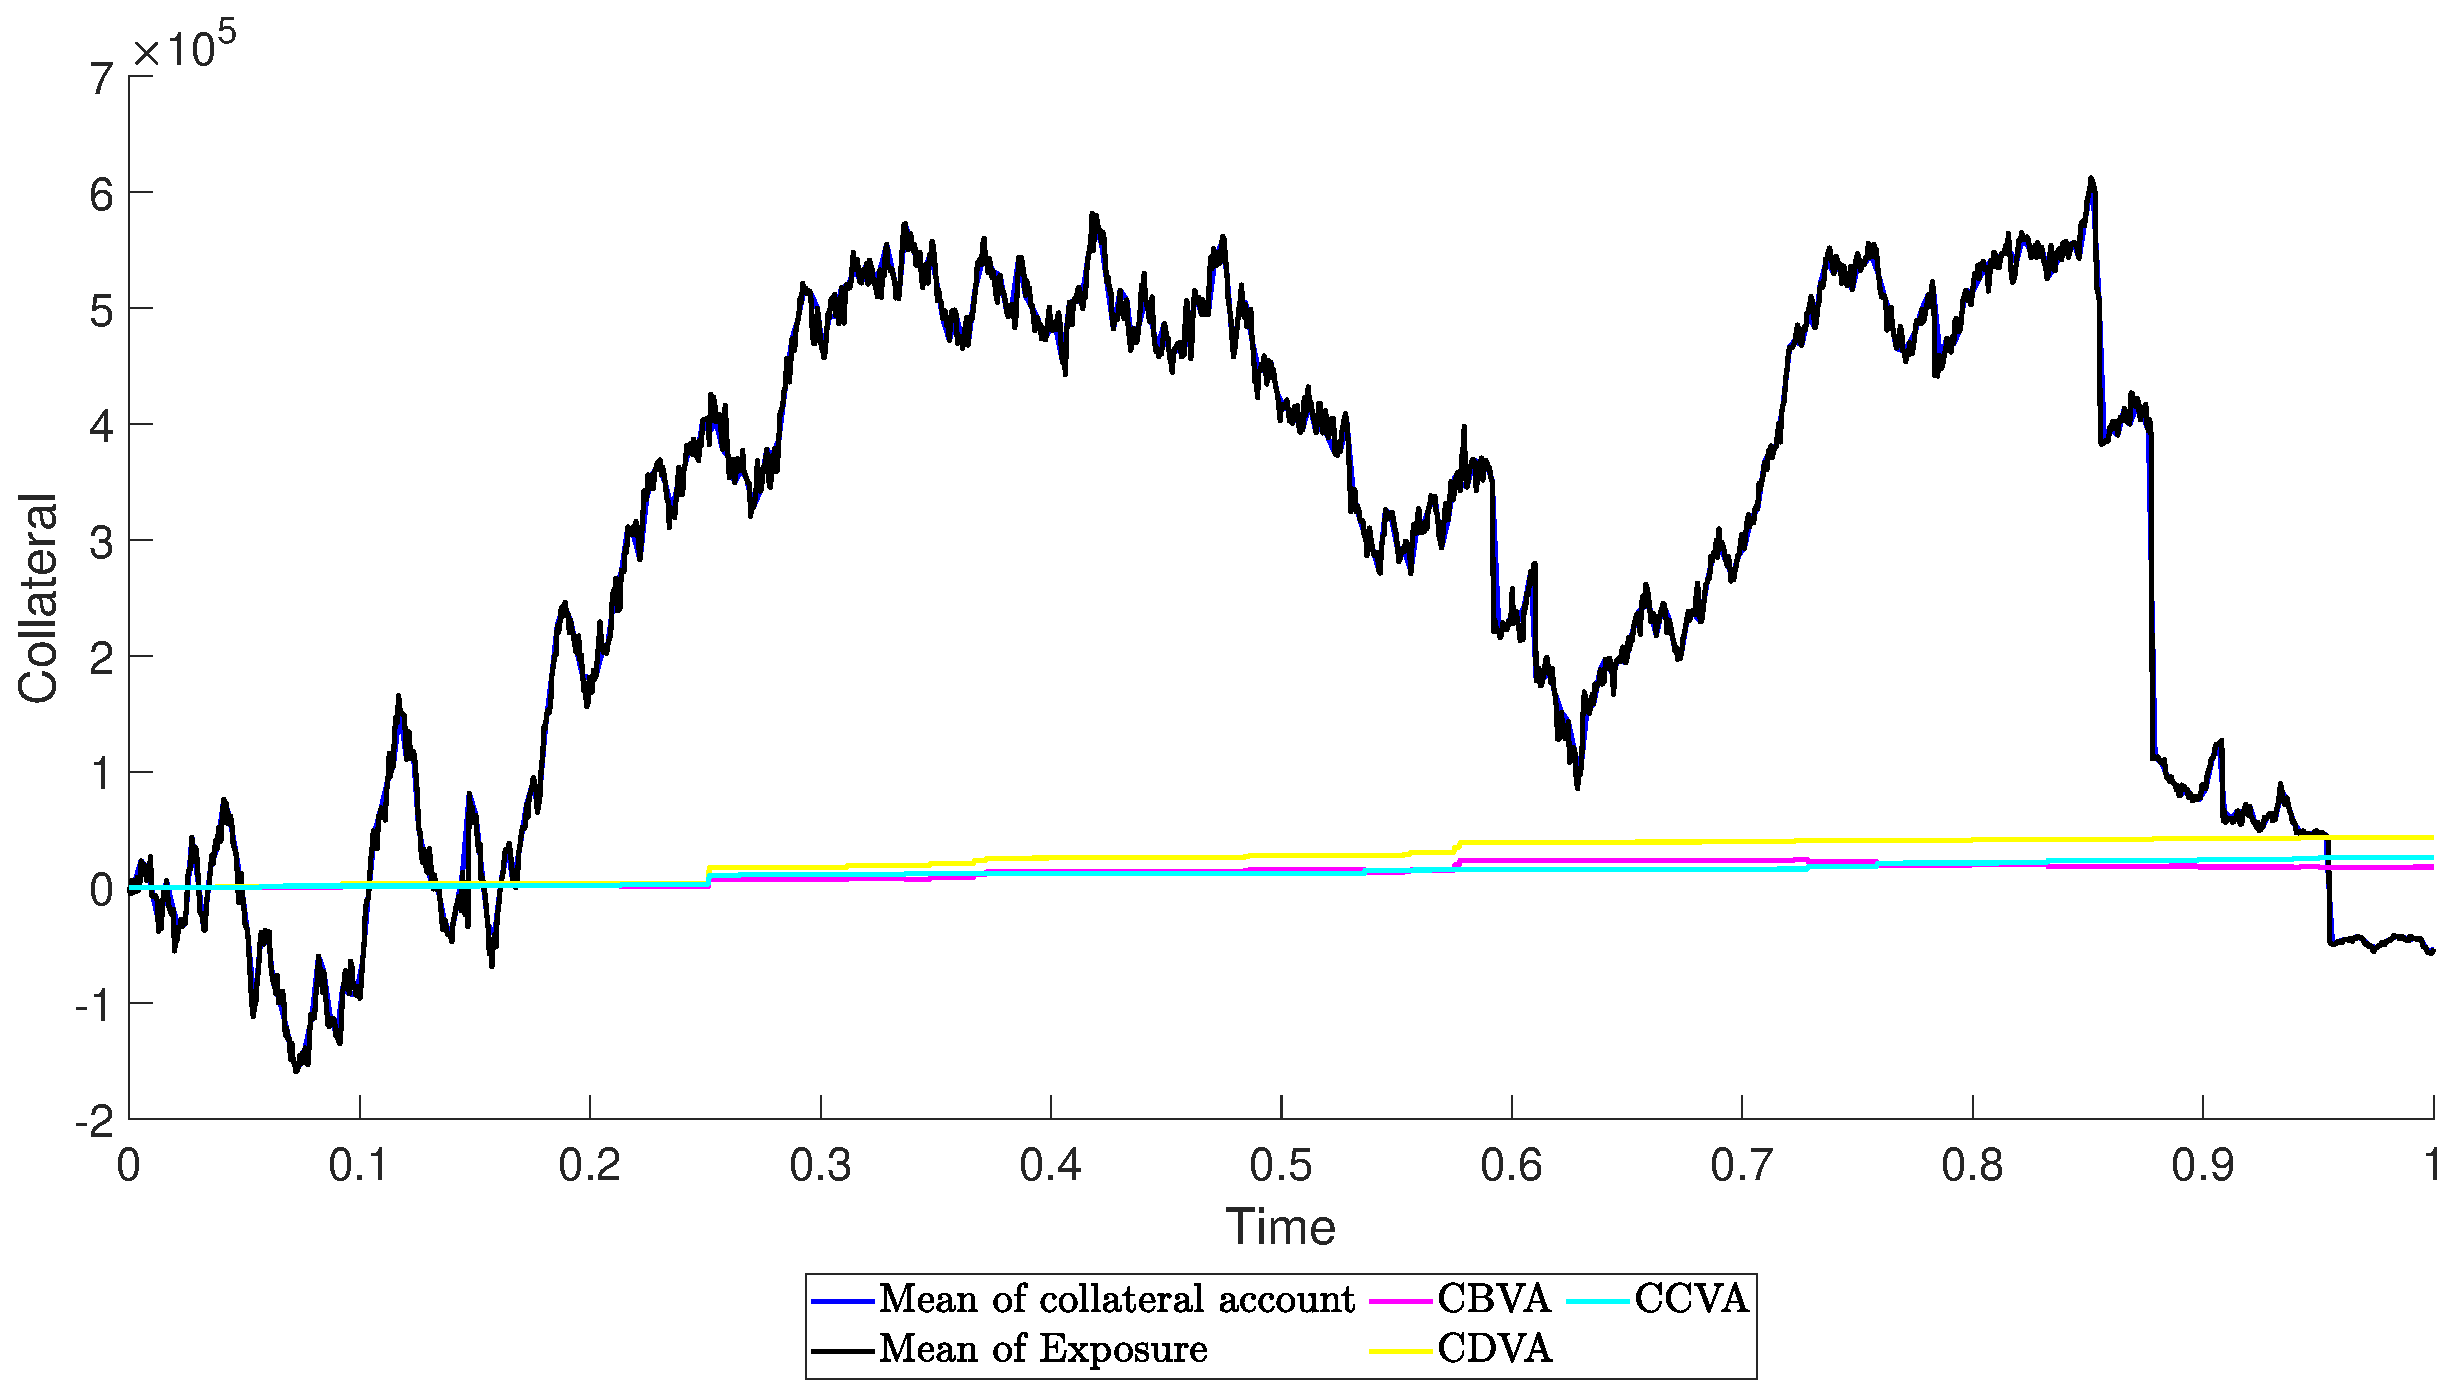
\includegraphics[width=.95\columnwidth]{CVAPC/CVAPC_FOBB_1}
\end{landscape}

\subsection{Rating Model trajectories}
\subsubsection{Under $\mathbb{P}$}
	\begin{landscape}
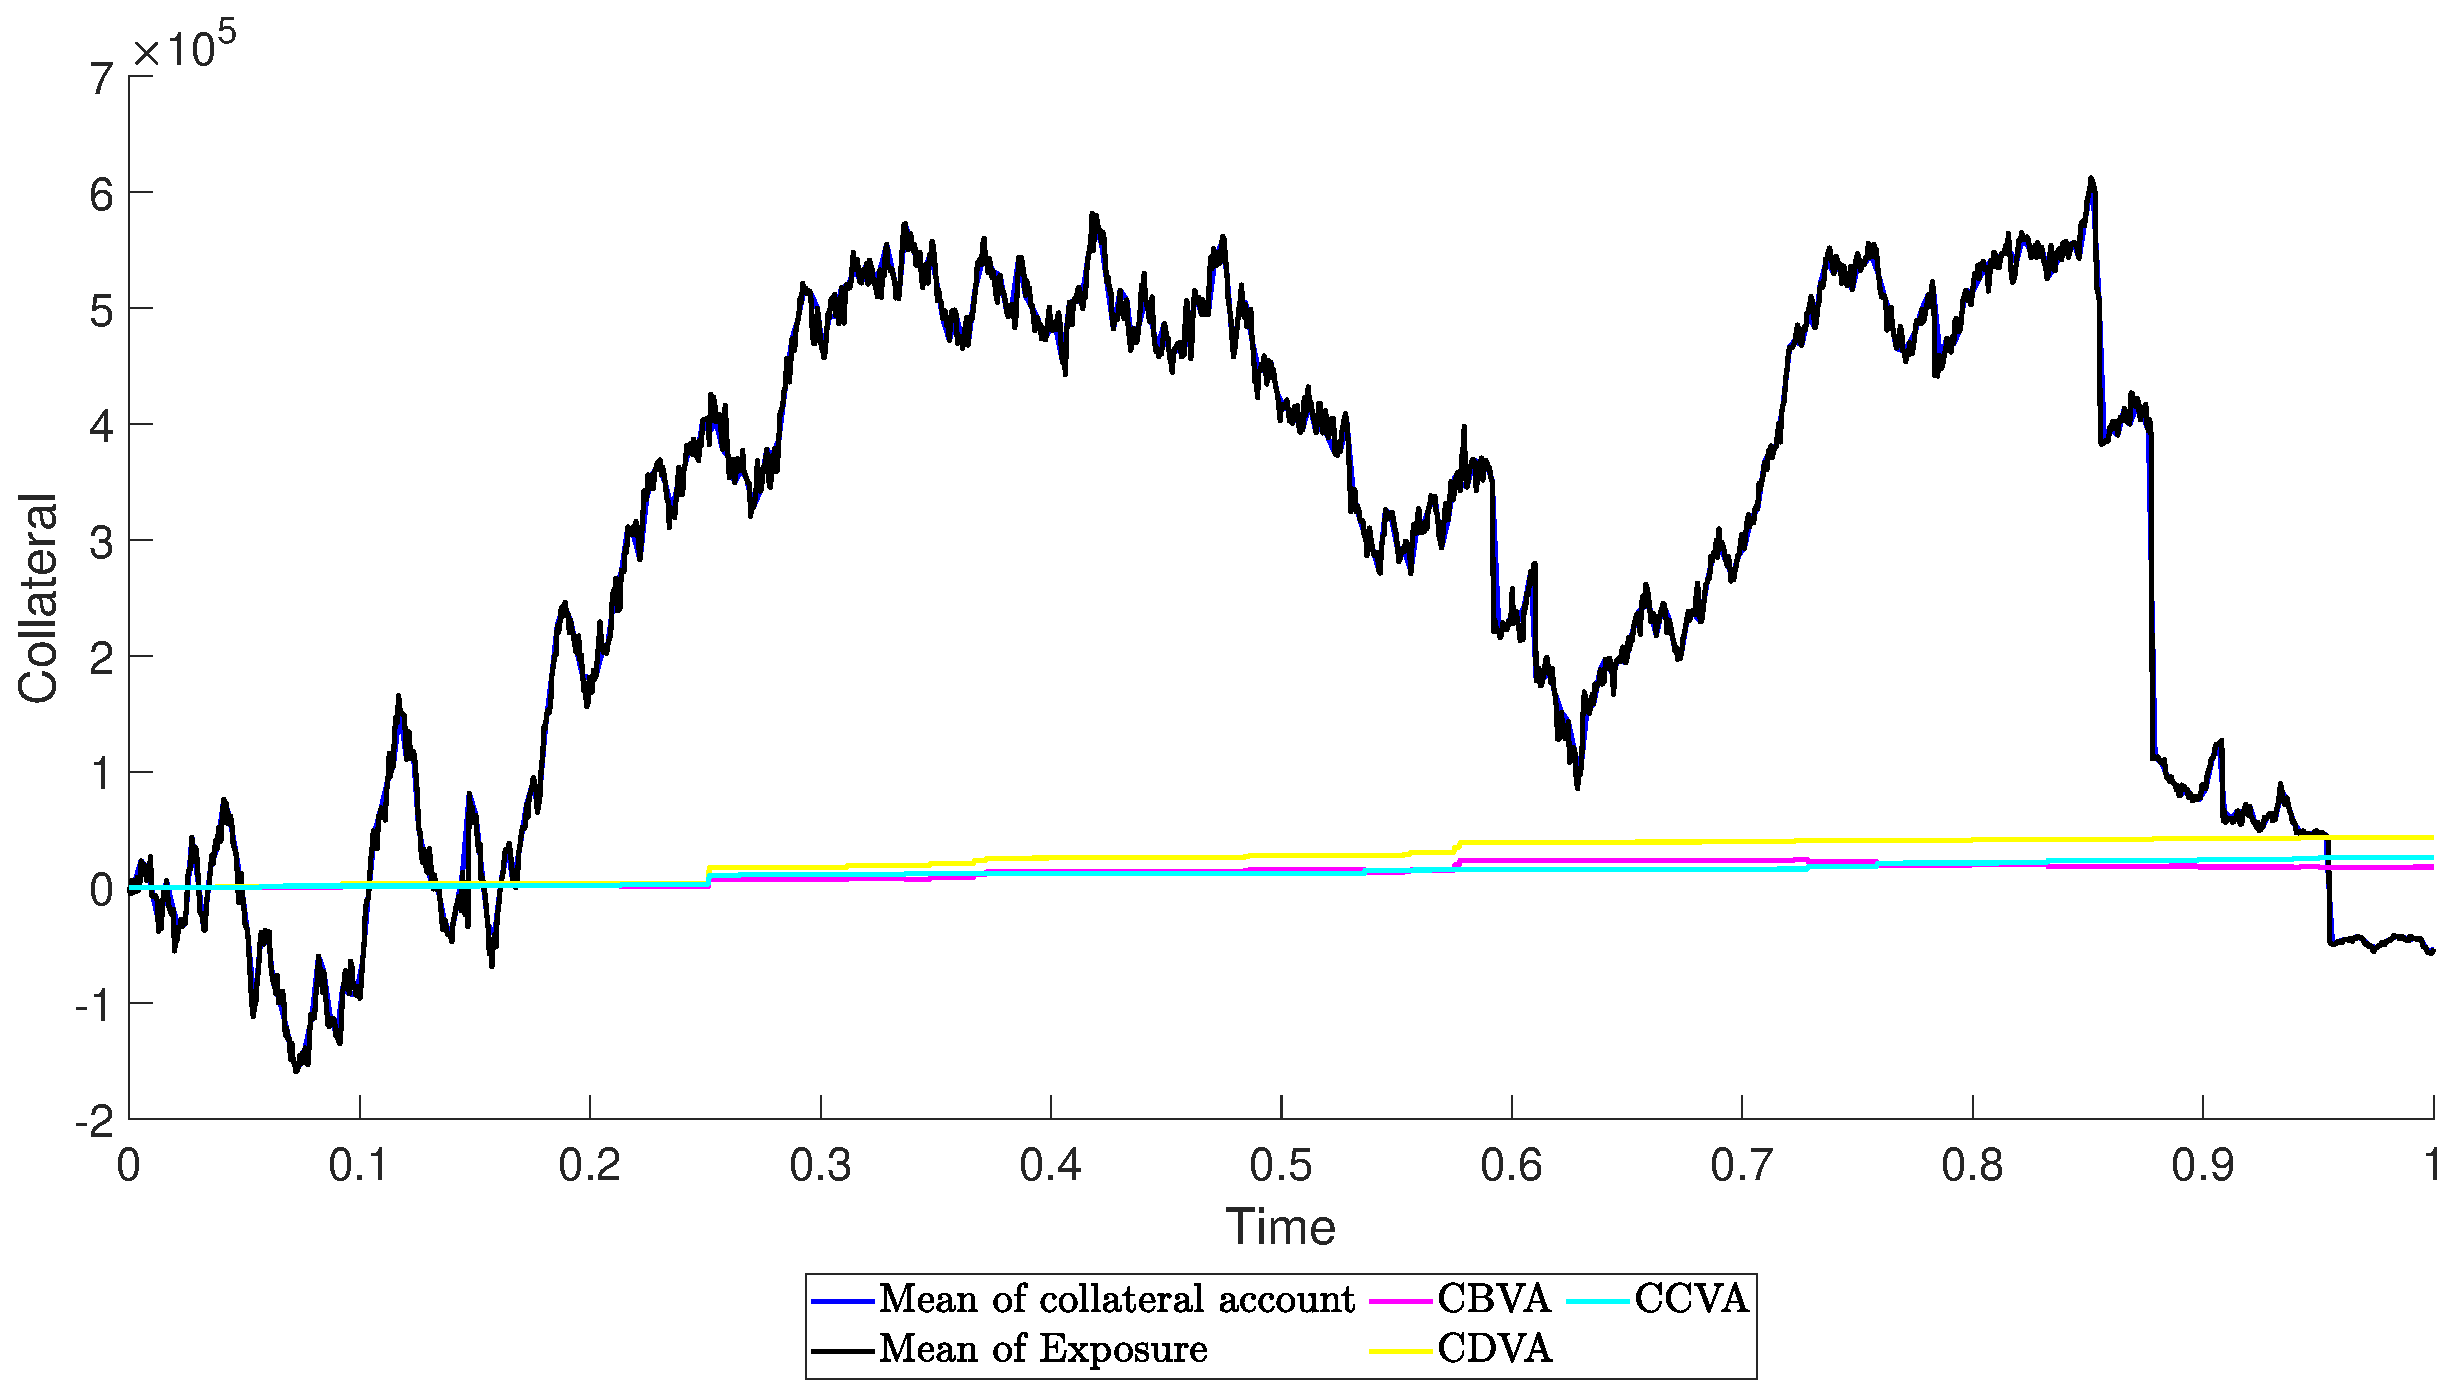
\includegraphics[width=.95\columnwidth]{CVAPC/CVAPC_FOBB_1}
\end{landscape}

\subsubsection{Under $\mathbb{Q}$}
	\begin{landscape}
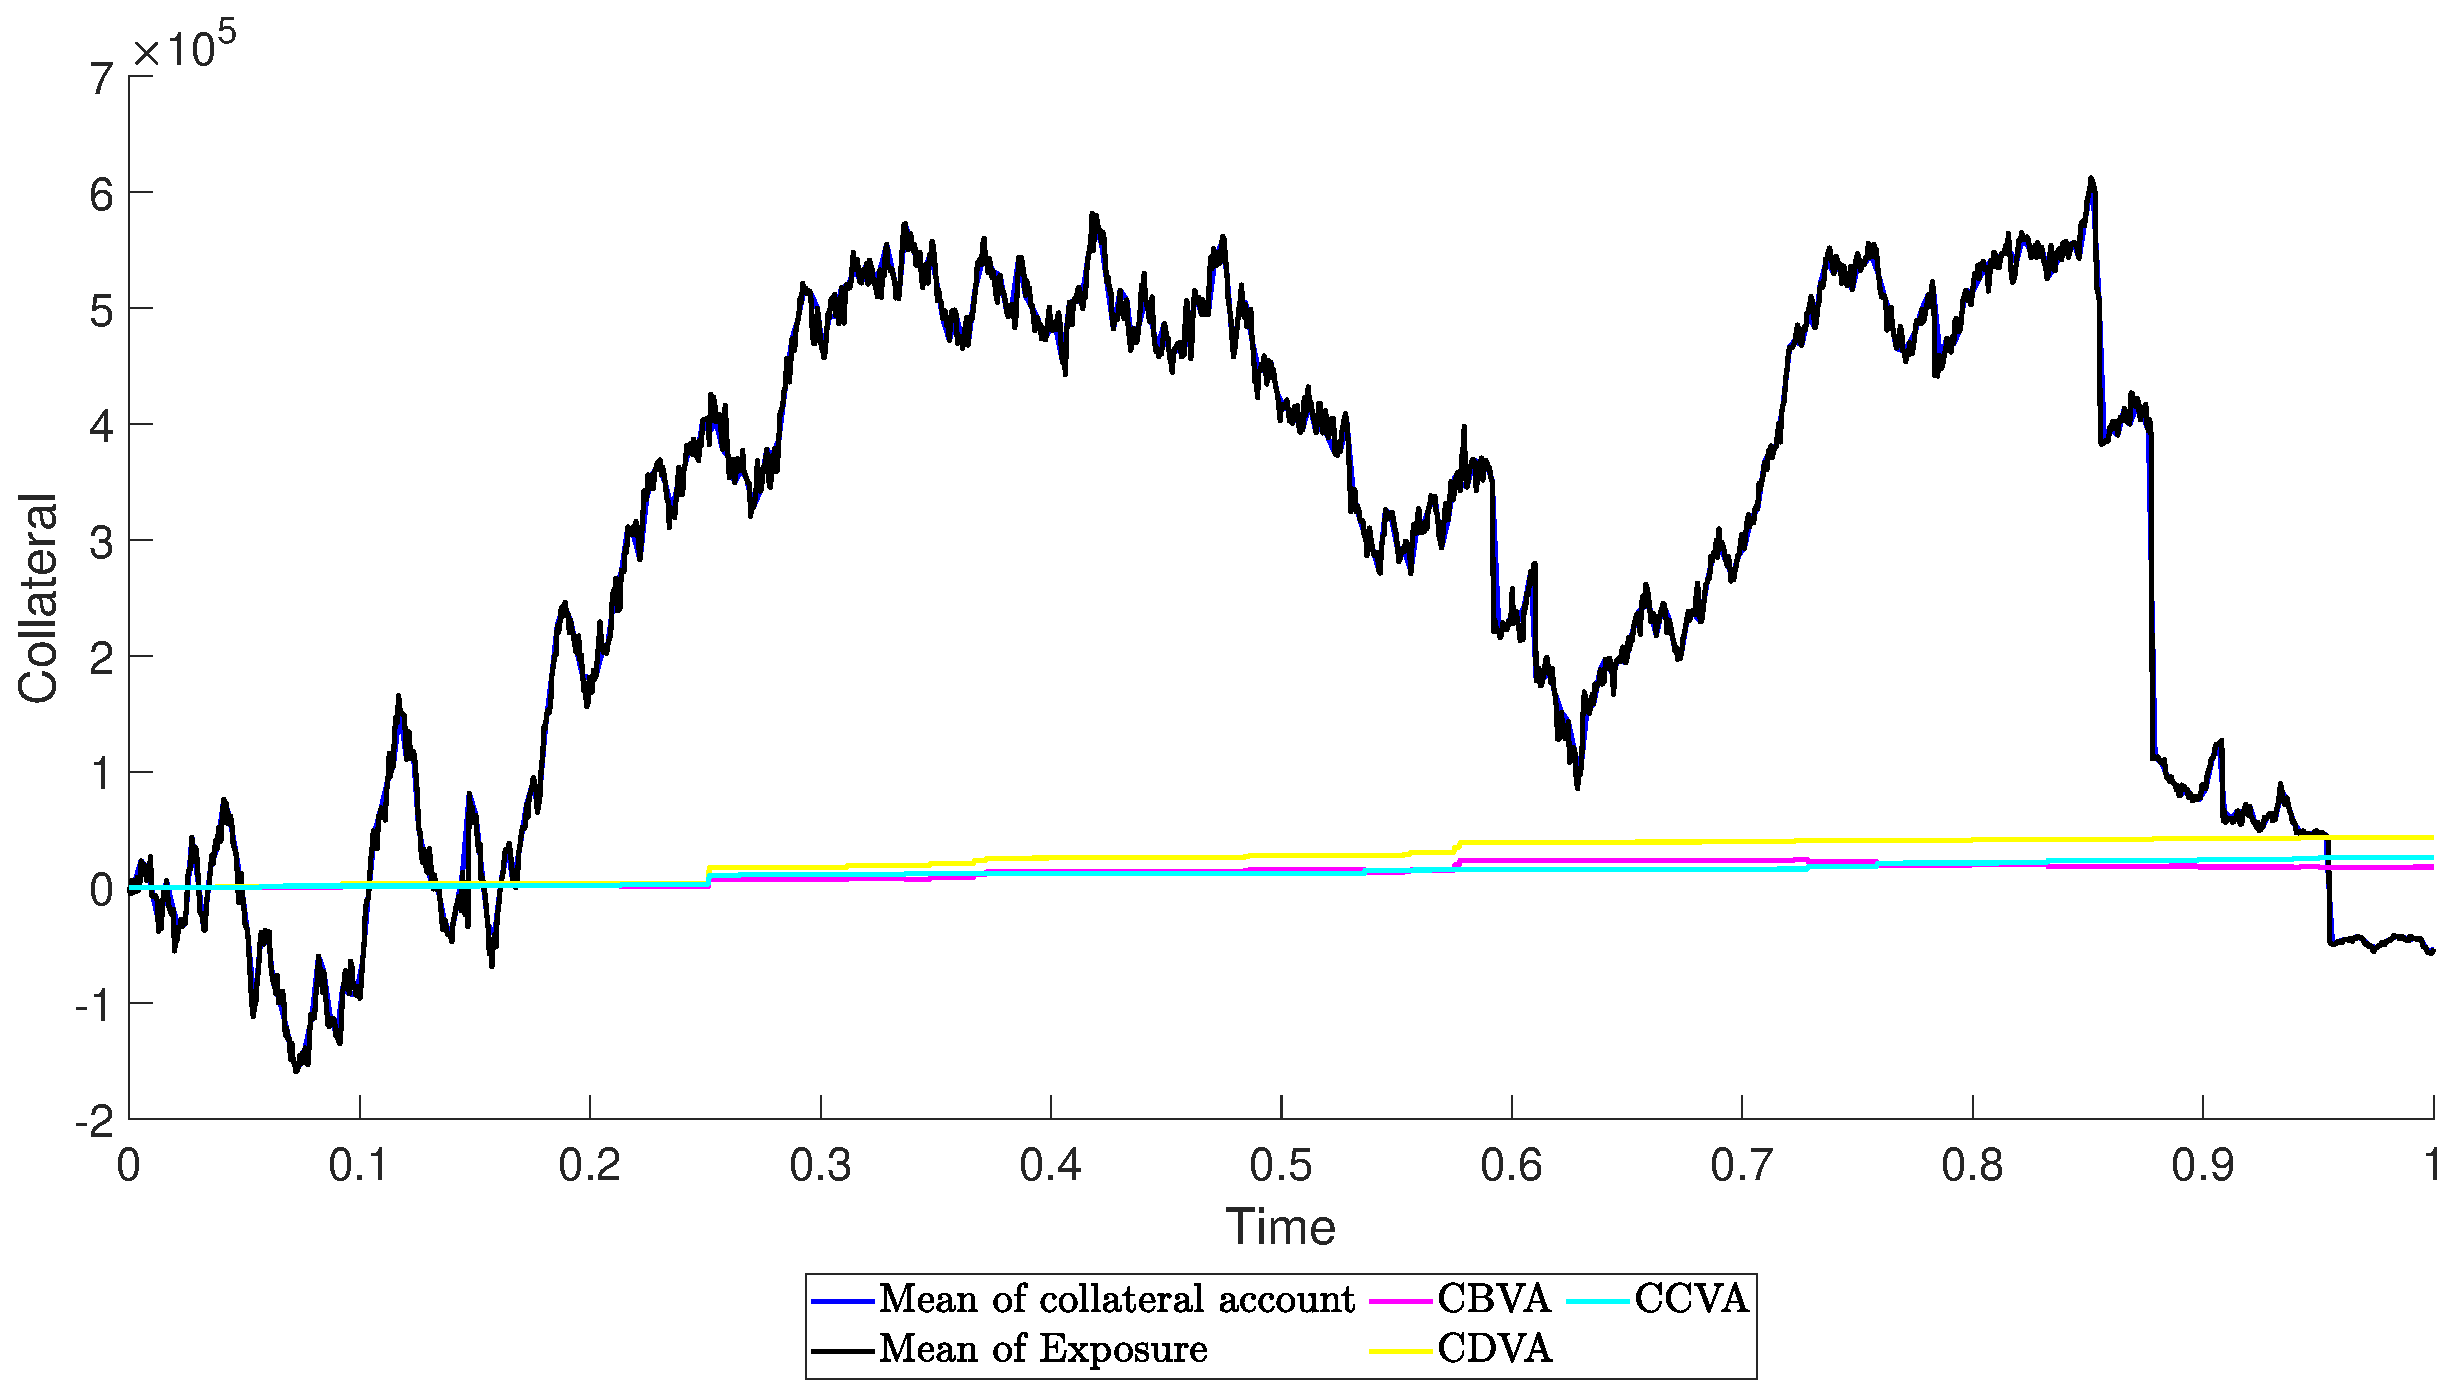
\includegraphics[width=.95\columnwidth]{CVAPC/CVAPC_FOBB_1}
\end{landscape}

\appendix
\section{Rating Matrices}
	\newcommand{\ratingMatricesMarketFOBBOne}{
\begin{tabular}{|c|*{7}{c}|}
\hline
\diagbox{From}{To} & F1+ & F1 & F2 & F3 & B & C & D\\ \hline
F1+ & $98.840$\,\% & $0.610$\,\% & $0.020$\,\% & $0.000$\,\% & $0.000$\,\% & $0.000$\,\% & $0.000$\,\% \\
F1 & $0.260$\,\% & $98.740$\,\% & $0.620$\,\% & $0.030$\,\% & $0.000$\,\% & $0.000$\,\% & $0.000$\,\% \\
F2 & $0.030$\,\% & $0.280$\,\% & $98.610$\,\% & $0.510$\,\% & $0.090$\,\% & $0.000$\,\% & $0.000$\,\% \\
F3 & $0.010$\,\% & $0.040$\,\% & $0.720$\,\% & $97.680$\,\% & $0.800$\,\% & $0.020$\,\% & $0.010$\,\% \\
B & $0.000$\,\% & $0.000$\,\% & $0.040$\,\% & $0.340$\,\% & $98.380$\,\% & $0.360$\,\% & $0.030$\,\% \\
C & $0.000$\,\% & $0.000$\,\% & $0.000$\,\% & $0.000$\,\% & $2.830$\,\% & $93.350$\,\% & $1.870$\,\% \\
D & $0.000$\,\% & $0.000$\,\% & $0.000$\,\% & $0.000$\,\% & $0.000$\,\% & $0.000$\,\% & $100.000$\,\% 
\\\hline
\end{tabular}
}
\newcommand{\ratingMatricesMarketFOBBOneCaption}{
\caption{Market at 0.083}}
\newcommand{\ratingMatricesMarketFOBBTwo}{
\begin{tabular}{|c|*{7}{c}|}
\hline
\diagbox{From}{To} & F1+ & F1 & F2 & F3 & B & C & D\\ \hline
F1+ & $96.550$\,\% & $1.790$\,\% & $0.080$\,\% & $0.020$\,\% & $0.000$\,\% & $0.000$\,\% & $0.000$\,\% \\
F1 & $0.750$\,\% & $96.230$\,\% & $1.790$\,\% & $0.090$\,\% & $0.030$\,\% & $0.000$\,\% & $0.010$\,\% \\
F2 & $0.090$\,\% & $0.830$\,\% & $95.870$\,\% & $1.470$\,\% & $0.300$\,\% & $0.010$\,\% & $0.020$\,\% \\
F3 & $0.040$\,\% & $0.120$\,\% & $2.170$\,\% & $93.140$\,\% & $2.280$\,\% & $0.040$\,\% & $0.020$\,\% \\
B & $0.000$\,\% & $0.010$\,\% & $0.130$\,\% & $1.030$\,\% & $95.170$\,\% & $1.000$\,\% & $0.140$\,\% \\
C & $0.000$\,\% & $0.000$\,\% & $0.000$\,\% & $0.000$\,\% & $8.520$\,\% & $81.470$\,\% & $4.760$\,\% \\
D & $0.000$\,\% & $0.000$\,\% & $0.000$\,\% & $0.000$\,\% & $0.000$\,\% & $0.000$\,\% & $100.000$\,\% 
\\\hline
\end{tabular}
}
\newcommand{\ratingMatricesMarketFOBBTwoCaption}{
\caption{Market at 0.250}}
\newcommand{\ratingMatricesMarketFOBBThree}{
\begin{tabular}{|c|*{7}{c}|}
\hline
\diagbox{From}{To} & F1+ & F1 & F2 & F3 & B & C & D\\ \hline
F1+ & $93.190$\,\% & $3.460$\,\% & $0.200$\,\% & $0.040$\,\% & $0.010$\,\% & $0.000$\,\% & $0.020$\,\% \\
F1 & $1.470$\,\% & $92.610$\,\% & $3.410$\,\% & $0.210$\,\% & $0.090$\,\% & $0.000$\,\% & $0.020$\,\% \\
F2 & $0.160$\,\% & $1.650$\,\% & $91.900$\,\% & $2.730$\,\% & $0.620$\,\% & $0.040$\,\% & $0.030$\,\% \\
F3 & $0.080$\,\% & $0.220$\,\% & $4.210$\,\% & $86.760$\,\% & $4.140$\,\% & $0.080$\,\% & $0.060$\,\% \\
B & $0.000$\,\% & $0.020$\,\% & $0.250$\,\% & $2.060$\,\% & $90.460$\,\% & $1.740$\,\% & $0.380$\,\% \\
C & $0.000$\,\% & $0.000$\,\% & $0.000$\,\% & $0.000$\,\% & $16.870$\,\% & $66.140$\,\% & $7.580$\,\% \\
D & $0.000$\,\% & $0.000$\,\% & $0.000$\,\% & $0.000$\,\% & $0.000$\,\% & $0.000$\,\% & $100.000$\,\% 
\\\hline
\end{tabular}
}
\newcommand{\ratingMatricesMarketFOBBThreeCaption}{
\caption{Market at 0.500}}
\newcommand{\ratingMatricesMarketFOBBFour}{
\begin{tabular}{|c|*{7}{c}|}
\hline
\diagbox{From}{To} & F1+ & F1 & F2 & F3 & B & C & D\\ \hline
F1+ & $86.950$\,\% & $6.350$\,\% & $0.550$\,\% & $0.090$\,\% & $0.040$\,\% & $0.000$\,\% & $0.050$\,\% \\
F1 & $2.720$\,\% & $85.850$\,\% & $6.200$\,\% & $0.500$\,\% & $0.290$\,\% & $0.000$\,\% & $0.050$\,\% \\
F2 & $0.260$\,\% & $3.180$\,\% & $84.420$\,\% & $4.660$\,\% & $1.370$\,\% & $0.100$\,\% & $0.090$\,\% \\
F3 & $0.190$\,\% & $0.400$\,\% & $8.250$\,\% & $75.270$\,\% & $6.540$\,\% & $0.190$\,\% & $0.230$\,\% \\
B & $0.000$\,\% & $0.030$\,\% & $0.460$\,\% & $4.040$\,\% & $81.890$\,\% & $2.780$\,\% & $0.950$\,\% \\
C & $0.000$\,\% & $0.000$\,\% & $0.000$\,\% & $0.000$\,\% & $31.880$\,\% & $42.400$\,\% & $10.440$\,\% \\
D & $0.000$\,\% & $0.000$\,\% & $0.000$\,\% & $0.000$\,\% & $0.000$\,\% & $0.000$\,\% & $100.000$\,\% 
\\\hline
\end{tabular}
}
\newcommand{\ratingMatricesMarketFOBBFourCaption}{
\caption{Market at 1.000}}
\newcommand{\ratingMatricesAdjustedFOBBOne}{
\begin{tabular}{|c|*{7}{c}|}
\hline
\diagbox{From}{To} & F1+ & F1 & F2 & F3 & B & C & D\\ \hline
F1+ & $99.367$\,\% & $0.613$\,\% & $0.020$\,\% & $0.000$\,\% & $0.000$\,\% & $0.000$\,\% & $0.000$\,\% \\
F1 & $0.261$\,\% & $99.087$\,\% & $0.622$\,\% & $0.030$\,\% & $0.000$\,\% & $0.000$\,\% & $0.000$\,\% \\
F2 & $0.030$\,\% & $0.281$\,\% & $99.086$\,\% & $0.512$\,\% & $0.090$\,\% & $0.000$\,\% & $0.000$\,\% \\
F3 & $0.010$\,\% & $0.040$\,\% & $0.725$\,\% & $98.388$\,\% & $0.806$\,\% & $0.020$\,\% & $0.010$\,\% \\
B & $0.000$\,\% & $0.000$\,\% & $0.040$\,\% & $0.343$\,\% & $99.223$\,\% & $0.363$\,\% & $0.030$\,\% \\
C & $0.000$\,\% & $0.000$\,\% & $0.000$\,\% & $0.000$\,\% & $2.886$\,\% & $95.207$\,\% & $1.907$\,\% \\
D & $0.000$\,\% & $0.000$\,\% & $0.000$\,\% & $0.000$\,\% & $0.000$\,\% & $0.000$\,\% & $100.000$\,\% 
\\\hline
\end{tabular}
}
\newcommand{\ratingMatricesAdjustedFOBBOneCaption}{
\caption{Adjusted at 0.083}}
\newcommand{\ratingMatricesAdjustedFOBBTwo}{
\begin{tabular}{|c|*{7}{c}|}
\hline
\diagbox{From}{To} & F1+ & F1 & F2 & F3 & B & C & D\\ \hline
F1+ & $98.080$\,\% & $1.818$\,\% & $0.081$\,\% & $0.020$\,\% & $0.000$\,\% & $0.000$\,\% & $0.000$\,\% \\
F1 & $0.758$\,\% & $97.300$\,\% & $1.810$\,\% & $0.091$\,\% & $0.030$\,\% & $0.000$\,\% & $0.010$\,\% \\
F2 & $0.091$\,\% & $0.842$\,\% & $97.241$\,\% & $1.491$\,\% & $0.304$\,\% & $0.010$\,\% & $0.020$\,\% \\
F3 & $0.041$\,\% & $0.123$\,\% & $2.219$\,\% & $95.225$\,\% & $2.331$\,\% & $0.041$\,\% & $0.020$\,\% \\
B & $0.000$\,\% & $0.010$\,\% & $0.133$\,\% & $1.057$\,\% & $97.630$\,\% & $1.026$\,\% & $0.144$\,\% \\
C & $0.000$\,\% & $0.000$\,\% & $0.000$\,\% & $0.000$\,\% & $8.992$\,\% & $85.984$\,\% & $5.024$\,\% \\
D & $0.000$\,\% & $0.000$\,\% & $0.000$\,\% & $0.000$\,\% & $0.000$\,\% & $0.000$\,\% & $100.000$\,\% 
\\\hline
\end{tabular}
}
\newcommand{\ratingMatricesAdjustedFOBBTwoCaption}{
\caption{Adjusted at 0.250}}
\newcommand{\ratingMatricesAdjustedFOBBThree}{
\begin{tabular}{|c|*{7}{c}|}
\hline
\diagbox{From}{To} & F1+ & F1 & F2 & F3 & B & C & D\\ \hline
F1+ & $96.151$\,\% & $3.570$\,\% & $0.206$\,\% & $0.041$\,\% & $0.010$\,\% & $0.000$\,\% & $0.021$\,\% \\
F1 & $1.503$\,\% & $94.684$\,\% & $3.486$\,\% & $0.215$\,\% & $0.092$\,\% & $0.000$\,\% & $0.020$\,\% \\
F2 & $0.165$\,\% & $1.699$\,\% & $94.615$\,\% & $2.811$\,\% & $0.638$\,\% & $0.041$\,\% & $0.031$\,\% \\
F3 & $0.084$\,\% & $0.230$\,\% & $4.406$\,\% & $90.801$\,\% & $4.333$\,\% & $0.084$\,\% & $0.063$\,\% \\
B & $0.000$\,\% & $0.021$\,\% & $0.263$\,\% & $2.170$\,\% & $95.311$\,\% & $1.833$\,\% & $0.400$\,\% \\
C & $0.000$\,\% & $0.000$\,\% & $0.000$\,\% & $0.000$\,\% & $18.622$\,\% & $73.010$\,\% & $8.367$\,\% \\
D & $0.000$\,\% & $0.000$\,\% & $0.000$\,\% & $0.000$\,\% & $0.000$\,\% & $0.000$\,\% & $100.000$\,\% 
\\\hline
\end{tabular}
}
\newcommand{\ratingMatricesAdjustedFOBBThreeCaption}{
\caption{Adjusted at 0.500}}
\newcommand{\ratingMatricesAdjustedFOBBFour}{
\begin{tabular}{|c|*{7}{c}|}
\hline
\diagbox{From}{To} & F1+ & F1 & F2 & F3 & B & C & D\\ \hline
F1+ & $92.470$\,\% & $6.753$\,\% & $0.585$\,\% & $0.096$\,\% & $0.043$\,\% & $0.000$\,\% & $0.053$\,\% \\
F1 & $2.845$\,\% & $89.792$\,\% & $6.485$\,\% & $0.523$\,\% & $0.303$\,\% & $0.000$\,\% & $0.052$\,\% \\
F2 & $0.276$\,\% & $3.380$\,\% & $89.732$\,\% & $4.953$\,\% & $1.456$\,\% & $0.106$\,\% & $0.096$\,\% \\
F3 & $0.209$\,\% & $0.439$\,\% & $9.059$\,\% & $82.651$\,\% & $7.181$\,\% & $0.209$\,\% & $0.253$\,\% \\
B & $0.000$\,\% & $0.033$\,\% & $0.510$\,\% & $4.481$\,\% & $90.837$\,\% & $3.084$\,\% & $1.054$\,\% \\
C & $0.000$\,\% & $0.000$\,\% & $0.000$\,\% & $0.000$\,\% & $37.630$\,\% & $50.047$\,\% & $12.323$\,\% \\
D & $0.000$\,\% & $0.000$\,\% & $0.000$\,\% & $0.000$\,\% & $0.000$\,\% & $0.000$\,\% & $100.000$\,\% 
\\\hline
\end{tabular}
}
\newcommand{\ratingMatricesAdjustedFOBBFourCaption}{
\caption{Adjusted at 1.000}}
\newcommand{\ratingMatricesAnalyticPFOBBOne}{
\begin{tabular}{|c|*{7}{c}|}
\hline
\diagbox{From}{To} & F1+ & F1 & F2 & F3 & B & C & D\\ \hline
F1+ & $99.366$\,\% & $0.613$\,\% & $0.020$\,\% & $0.000$\,\% & $0.000$\,\% & $0.000$\,\% & $0.000$\,\% \\
F1 & $0.261$\,\% & $99.086$\,\% & $0.622$\,\% & $0.030$\,\% & $0.000$\,\% & $0.000$\,\% & $0.000$\,\% \\
F2 & $0.030$\,\% & $0.281$\,\% & $99.085$\,\% & $0.512$\,\% & $0.090$\,\% & $0.000$\,\% & $0.000$\,\% \\
F3 & $0.010$\,\% & $0.040$\,\% & $0.725$\,\% & $98.388$\,\% & $0.806$\,\% & $0.020$\,\% & $0.010$\,\% \\
B & $0.000$\,\% & $0.000$\,\% & $0.040$\,\% & $0.343$\,\% & $99.223$\,\% & $0.363$\,\% & $0.030$\,\% \\
C & $0.000$\,\% & $0.000$\,\% & $0.001$\,\% & $0.005$\,\% & $2.886$\,\% & $95.201$\,\% & $1.907$\,\% \\
D & $0.000$\,\% & $0.000$\,\% & $0.000$\,\% & $0.000$\,\% & $0.000$\,\% & $0.000$\,\% & $100.000$\,\% 
\\\hline
\end{tabular}
}
\newcommand{\ratingMatricesAnalyticPFOBBOneCaption}{
\caption{AnalyticP at 0.083}}
\newcommand{\ratingMatricesAnalyticPFOBBTwo}{
\begin{tabular}{|c|*{7}{c}|}
\hline
\diagbox{From}{To} & F1+ & F1 & F2 & F3 & B & C & D\\ \hline
F1+ & $98.079$\,\% & $1.818$\,\% & $0.081$\,\% & $0.020$\,\% & $0.001$\,\% & $0.000$\,\% & $0.000$\,\% \\
F1 & $0.758$\,\% & $97.300$\,\% & $1.810$\,\% & $0.091$\,\% & $0.030$\,\% & $0.000$\,\% & $0.010$\,\% \\
F2 & $0.091$\,\% & $0.842$\,\% & $97.241$\,\% & $1.491$\,\% & $0.304$\,\% & $0.010$\,\% & $0.020$\,\% \\
F3 & $0.041$\,\% & $0.123$\,\% & $2.219$\,\% & $95.225$\,\% & $2.331$\,\% & $0.041$\,\% & $0.020$\,\% \\
B & $0.000$\,\% & $0.010$\,\% & $0.133$\,\% & $1.057$\,\% & $97.630$\,\% & $1.025$\,\% & $0.144$\,\% \\
C & $0.000$\,\% & $0.001$\,\% & $0.006$\,\% & $0.049$\,\% & $8.991$\,\% & $85.931$\,\% & $5.023$\,\% \\
D & $0.000$\,\% & $0.000$\,\% & $0.000$\,\% & $0.000$\,\% & $0.000$\,\% & $0.000$\,\% & $100.000$\,\% 
\\\hline
\end{tabular}
}
\newcommand{\ratingMatricesAnalyticPFOBBTwoCaption}{
\caption{AnalyticP at 0.250}}
\newcommand{\ratingMatricesAnalyticPFOBBThree}{
\begin{tabular}{|c|*{7}{c}|}
\hline
\diagbox{From}{To} & F1+ & F1 & F2 & F3 & B & C & D\\ \hline
F1+ & $96.151$\,\% & $3.570$\,\% & $0.206$\,\% & $0.041$\,\% & $0.010$\,\% & $0.000$\,\% & $0.021$\,\% \\
F1 & $1.503$\,\% & $94.682$\,\% & $3.486$\,\% & $0.215$\,\% & $0.092$\,\% & $0.002$\,\% & $0.020$\,\% \\
F2 & $0.165$\,\% & $1.699$\,\% & $94.615$\,\% & $2.811$\,\% & $0.638$\,\% & $0.041$\,\% & $0.031$\,\% \\
F3 & $0.084$\,\% & $0.230$\,\% & $4.406$\,\% & $90.801$\,\% & $4.333$\,\% & $0.084$\,\% & $0.063$\,\% \\
B & $0.001$\,\% & $0.021$\,\% & $0.264$\,\% & $2.174$\,\% & $95.310$\,\% & $1.829$\,\% & $0.400$\,\% \\
C & $0.000$\,\% & $0.002$\,\% & $0.023$\,\% & $0.216$\,\% & $18.610$\,\% & $72.787$\,\% & $8.362$\,\% \\
D & $0.000$\,\% & $0.000$\,\% & $0.000$\,\% & $0.000$\,\% & $0.000$\,\% & $0.000$\,\% & $100.000$\,\% 
\\\hline
\end{tabular}
}
\newcommand{\ratingMatricesAnalyticPFOBBThreeCaption}{
\caption{AnalyticP at 0.500}}
\newcommand{\ratingMatricesAnalyticPFOBBFour}{
\begin{tabular}{|c|*{7}{c}|}
\hline
\diagbox{From}{To} & F1+ & F1 & F2 & F3 & B & C & D\\ \hline
F1+ & $92.470$\,\% & $6.753$\,\% & $0.585$\,\% & $0.096$\,\% & $0.043$\,\% & $0.001$\,\% & $0.053$\,\% \\
F1 & $2.845$\,\% & $89.782$\,\% & $6.485$\,\% & $0.523$\,\% & $0.305$\,\% & $0.008$\,\% & $0.053$\,\% \\
F2 & $0.276$\,\% & $3.380$\,\% & $89.732$\,\% & $4.954$\,\% & $1.456$\,\% & $0.105$\,\% & $0.096$\,\% \\
F3 & $0.209$\,\% & $0.439$\,\% & $9.059$\,\% & $82.653$\,\% & $7.181$\,\% & $0.206$\,\% & $0.252$\,\% \\
B & $0.007$\,\% & $0.034$\,\% & $0.513$\,\% & $4.522$\,\% & $90.826$\,\% & $3.046$\,\% & $1.053$\,\% \\
C & $0.003$\,\% & $0.004$\,\% & $0.076$\,\% & $0.989$\,\% & $37.477$\,\% & $49.160$\,\% & $12.292$\,\% \\
D & $0.000$\,\% & $0.000$\,\% & $0.000$\,\% & $0.000$\,\% & $0.000$\,\% & $0.000$\,\% & $100.000$\,\% 
\\\hline
\end{tabular}
}
\newcommand{\ratingMatricesAnalyticPFOBBFourCaption}{
\caption{AnalyticP at 1.000}}
\newcommand{\ratingMatricesAnalyticQFOBBOne}{
\begin{tabular}{|c|*{7}{c}|}
\hline
\diagbox{From}{To} & F1+ & F1 & F2 & F3 & B & C & D\\ \hline
F1+ & $99.387$\,\% & $0.525$\,\% & $0.047$\,\% & $0.037$\,\% & $0.002$\,\% & $0.001$\,\% & $0.000$\,\% \\
F1 & $0.274$\,\% & $89.006$\,\% & $1.519$\,\% & $9.022$\,\% & $0.121$\,\% & $0.044$\,\% & $0.015$\,\% \\
F2 & $0.007$\,\% & $0.059$\,\% & $55.661$\,\% & $36.427$\,\% & $7.034$\,\% & $0.718$\,\% & $0.093$\,\% \\
F3 & $0.000$\,\% & $0.000$\,\% & $0.006$\,\% & $97.903$\,\% & $0.880$\,\% & $0.897$\,\% & $0.314$\,\% \\
B & $0.000$\,\% & $0.000$\,\% & $0.000$\,\% & $0.271$\,\% & $86.068$\,\% & $12.906$\,\% & $0.754$\,\% \\
C & $0.000$\,\% & $0.000$\,\% & $0.000$\,\% & $0.000$\,\% & $0.073$\,\% & $98.549$\,\% & $1.378$\,\% \\
D & $0.000$\,\% & $0.000$\,\% & $0.000$\,\% & $0.000$\,\% & $0.000$\,\% & $0.000$\,\% & $100.000$\,\% 
\\\hline
\end{tabular}
}
\newcommand{\ratingMatricesAnalyticQFOBBOneCaption}{
\caption{AnalyticQ at 0.083}}
\newcommand{\ratingMatricesAnalyticQFOBBTwo}{
\begin{tabular}{|c|*{7}{c}|}
\hline
\diagbox{From}{To} & F1+ & F1 & F2 & F3 & B & C & D\\ \hline
F1+ & $98.169$\,\% & $1.670$\,\% & $0.107$\,\% & $0.053$\,\% & $0.001$\,\% & $0.001$\,\% & $0.000$\,\% \\
F1 & $0.749$\,\% & $87.409$\,\% & $2.787$\,\% & $8.951$\,\% & $0.028$\,\% & $0.057$\,\% & $0.019$\,\% \\
F2 & $0.059$\,\% & $0.470$\,\% & $56.188$\,\% & $39.979$\,\% & $1.598$\,\% & $1.497$\,\% & $0.209$\,\% \\
F3 & $0.040$\,\% & $0.106$\,\% & $1.995$\,\% & $96.327$\,\% & $0.206$\,\% & $0.974$\,\% & $0.352$\,\% \\
B & $0.017$\,\% & $0.788$\,\% & $7.440$\,\% & $47.676$\,\% & $19.531$\,\% & $22.292$\,\% & $2.256$\,\% \\
C & $0.000$\,\% & $0.002$\,\% & $0.018$\,\% & $0.117$\,\% & $0.133$\,\% & $95.649$\,\% & $4.081$\,\% \\
D & $0.000$\,\% & $0.000$\,\% & $0.000$\,\% & $0.000$\,\% & $0.000$\,\% & $0.000$\,\% & $100.000$\,\% 
\\\hline
\end{tabular}
}
\newcommand{\ratingMatricesAnalyticQFOBBTwoCaption}{
\caption{AnalyticQ at 0.250}}
\newcommand{\ratingMatricesAnalyticQFOBBThree}{
\begin{tabular}{|c|*{7}{c}|}
\hline
\diagbox{From}{To} & F1+ & F1 & F2 & F3 & B & C & D\\ \hline
F1+ & $96.230$\,\% & $1.293$\,\% & $2.211$\,\% & $0.000$\,\% & $0.010$\,\% & $0.003$\,\% & $0.253$\,\% \\
F1 & $2.124$\,\% & $43.119$\,\% & $53.709$\,\% & $0.000$\,\% & $0.488$\,\% & $0.190$\,\% & $0.370$\,\% \\
F2 & $0.119$\,\% & $0.266$\,\% & $93.478$\,\% & $0.000$\,\% & $3.066$\,\% & $2.188$\,\% & $0.883$\,\% \\
F3 & $0.163$\,\% & $0.111$\,\% & $91.393$\,\% & $0.000$\,\% & $4.366$\,\% & $2.221$\,\% & $1.747$\,\% \\
B & $0.090$\,\% & $0.419$\,\% & $52.321$\,\% & $0.000$\,\% & $18.202$\,\% & $24.553$\,\% & $4.415$\,\% \\
C & $0.000$\,\% & $0.001$\,\% & $0.136$\,\% & $0.000$\,\% & $0.846$\,\% & $91.028$\,\% & $7.989$\,\% \\
D & $0.000$\,\% & $0.000$\,\% & $0.000$\,\% & $0.000$\,\% & $0.000$\,\% & $0.000$\,\% & $100.000$\,\% 
\\\hline
\end{tabular}
}
\newcommand{\ratingMatricesAnalyticQFOBBThreeCaption}{
\caption{AnalyticQ at 0.500}}
\newcommand{\ratingMatricesAnalyticQFOBBFour}{
\begin{tabular}{|c|*{7}{c}|}
\hline
\diagbox{From}{To} & F1+ & F1 & F2 & F3 & B & C & D\\ \hline
F1+ & $81.278$\,\% & $15.739$\,\% & $1.776$\,\% & $0.678$\,\% & $0.005$\,\% & $0.018$\,\% & $0.506$\,\% \\
F1 & $1.984$\,\% & $47.735$\,\% & $38.809$\,\% & $10.024$\,\% & $0.113$\,\% & $0.598$\,\% & $0.738$\,\% \\
F2 & $0.191$\,\% & $8.750$\,\% & $67.134$\,\% & $18.079$\,\% & $0.523$\,\% & $3.445$\,\% & $1.878$\,\% \\
F3 & $0.226$\,\% & $8.415$\,\% & $65.639$\,\% & $18.241$\,\% & $0.711$\,\% & $3.881$\,\% & $2.886$\,\% \\
B & $0.129$\,\% & $5.179$\,\% & $37.626$\,\% & $17.009$\,\% & $2.789$\,\% & $28.517$\,\% & $8.751$\,\% \\
C & $0.001$\,\% & $0.014$\,\% & $0.101$\,\% & $0.626$\,\% & $0.524$\,\% & $83.413$\,\% & $15.319$\,\% \\
D & $0.000$\,\% & $0.000$\,\% & $0.000$\,\% & $0.000$\,\% & $0.000$\,\% & $0.000$\,\% & $100.000$\,\% 
\\\hline
\end{tabular}
}
\newcommand{\ratingMatricesAnalyticQFOBBFourCaption}{
\caption{AnalyticQ at 1.000}}
\newcommand{\ratingMatricesEvoPFOBBOne}{
\begin{tabular}{|c|*{7}{c}|}
\hline
\diagbox{From}{To} & F1+ & F1 & F2 & F3 & B & C & D\\ \hline
F1+ & $99.366$\,\% & $0.613$\,\% & $0.020$\,\% & $0.000$\,\% & $0.000$\,\% & $0.000$\,\% & $0.000$\,\% \\
F1 & $0.261$\,\% & $99.086$\,\% & $0.622$\,\% & $0.030$\,\% & $0.000$\,\% & $0.000$\,\% & $0.000$\,\% \\
F2 & $0.030$\,\% & $0.281$\,\% & $99.085$\,\% & $0.513$\,\% & $0.090$\,\% & $0.000$\,\% & $0.000$\,\% \\
F3 & $0.010$\,\% & $0.040$\,\% & $0.725$\,\% & $98.388$\,\% & $0.806$\,\% & $0.020$\,\% & $0.010$\,\% \\
B & $0.000$\,\% & $0.000$\,\% & $0.040$\,\% & $0.343$\,\% & $99.223$\,\% & $0.363$\,\% & $0.030$\,\% \\
C & $0.000$\,\% & $0.000$\,\% & $0.001$\,\% & $0.005$\,\% & $2.887$\,\% & $95.200$\,\% & $1.907$\,\% \\
D & $0.000$\,\% & $0.000$\,\% & $0.000$\,\% & $0.000$\,\% & $0.000$\,\% & $0.000$\,\% & $100.000$\,\% 
\\\hline
\end{tabular}
}
\newcommand{\ratingMatricesEvoPFOBBOneCaption}{
\caption{EvoP at 0.083}}
\newcommand{\ratingMatricesEvoPFOBBTwo}{
\begin{tabular}{|c|*{7}{c}|}
\hline
\diagbox{From}{To} & F1+ & F1 & F2 & F3 & B & C & D\\ \hline
F1+ & $98.079$\,\% & $1.818$\,\% & $0.081$\,\% & $0.020$\,\% & $0.001$\,\% & $0.000$\,\% & $0.000$\,\% \\
F1 & $0.758$\,\% & $97.300$\,\% & $1.810$\,\% & $0.091$\,\% & $0.030$\,\% & $0.000$\,\% & $0.010$\,\% \\
F2 & $0.091$\,\% & $0.842$\,\% & $97.241$\,\% & $1.491$\,\% & $0.304$\,\% & $0.010$\,\% & $0.020$\,\% \\
F3 & $0.041$\,\% & $0.123$\,\% & $2.218$\,\% & $95.225$\,\% & $2.331$\,\% & $0.041$\,\% & $0.020$\,\% \\
B & $0.000$\,\% & $0.010$\,\% & $0.133$\,\% & $1.057$\,\% & $97.630$\,\% & $1.026$\,\% & $0.143$\,\% \\
C & $0.000$\,\% & $0.001$\,\% & $0.006$\,\% & $0.049$\,\% & $8.989$\,\% & $85.930$\,\% & $5.025$\,\% \\
D & $0.000$\,\% & $0.000$\,\% & $0.000$\,\% & $0.000$\,\% & $0.000$\,\% & $0.000$\,\% & $100.000$\,\% 
\\\hline
\end{tabular}
}
\newcommand{\ratingMatricesEvoPFOBBTwoCaption}{
\caption{EvoP at 0.250}}
\newcommand{\ratingMatricesEvoPFOBBThree}{
\begin{tabular}{|c|*{7}{c}|}
\hline
\diagbox{From}{To} & F1+ & F1 & F2 & F3 & B & C & D\\ \hline
F1+ & $96.151$\,\% & $3.570$\,\% & $0.206$\,\% & $0.041$\,\% & $0.010$\,\% & $0.000$\,\% & $0.021$\,\% \\
F1 & $1.503$\,\% & $94.682$\,\% & $3.487$\,\% & $0.215$\,\% & $0.092$\,\% & $0.002$\,\% & $0.020$\,\% \\
F2 & $0.165$\,\% & $1.699$\,\% & $94.615$\,\% & $2.811$\,\% & $0.638$\,\% & $0.041$\,\% & $0.031$\,\% \\
F3 & $0.084$\,\% & $0.230$\,\% & $4.406$\,\% & $90.800$\,\% & $4.334$\,\% & $0.084$\,\% & $0.063$\,\% \\
B & $0.001$\,\% & $0.021$\,\% & $0.264$\,\% & $2.174$\,\% & $95.310$\,\% & $1.830$\,\% & $0.400$\,\% \\
C & $0.000$\,\% & $0.002$\,\% & $0.023$\,\% & $0.216$\,\% & $18.606$\,\% & $72.786$\,\% & $8.367$\,\% \\
D & $0.000$\,\% & $0.000$\,\% & $0.000$\,\% & $0.000$\,\% & $0.000$\,\% & $0.000$\,\% & $100.000$\,\% 
\\\hline
\end{tabular}
}
\newcommand{\ratingMatricesEvoPFOBBThreeCaption}{
\caption{EvoP at 0.500}}
\newcommand{\ratingMatricesEvoPFOBBFour}{
\begin{tabular}{|c|*{7}{c}|}
\hline
\diagbox{From}{To} & F1+ & F1 & F2 & F3 & B & C & D\\ \hline
F1+ & $92.470$\,\% & $6.753$\,\% & $0.585$\,\% & $0.096$\,\% & $0.043$\,\% & $0.001$\,\% & $0.053$\,\% \\
F1 & $2.845$\,\% & $89.782$\,\% & $6.485$\,\% & $0.523$\,\% & $0.305$\,\% & $0.008$\,\% & $0.053$\,\% \\
F2 & $0.277$\,\% & $3.380$\,\% & $89.732$\,\% & $4.955$\,\% & $1.456$\,\% & $0.105$\,\% & $0.096$\,\% \\
F3 & $0.209$\,\% & $0.439$\,\% & $9.058$\,\% & $82.652$\,\% & $7.182$\,\% & $0.207$\,\% & $0.252$\,\% \\
B & $0.007$\,\% & $0.034$\,\% & $0.513$\,\% & $4.522$\,\% & $90.826$\,\% & $3.046$\,\% & $1.052$\,\% \\
C & $0.003$\,\% & $0.004$\,\% & $0.076$\,\% & $0.988$\,\% & $37.472$\,\% & $49.158$\,\% & $12.299$\,\% \\
D & $0.000$\,\% & $0.000$\,\% & $0.000$\,\% & $0.000$\,\% & $0.000$\,\% & $0.000$\,\% & $100.000$\,\% 
\\\hline
\end{tabular}
}
\newcommand{\ratingMatricesEvoPFOBBFourCaption}{
\caption{EvoP at 1.000}}
\newcommand{\ratingMatricesEvoQFOBBOne}{
\begin{tabular}{|c|*{7}{c}|}
\hline
\diagbox{From}{To} & F1+ & F1 & F2 & F3 & B & C & D\\ \hline
F1+ & $99.387$\,\% & $0.526$\,\% & $0.047$\,\% & $0.036$\,\% & $0.002$\,\% & $0.001$\,\% & $0.000$\,\% \\
F1 & $0.274$\,\% & $89.002$\,\% & $1.522$\,\% & $9.024$\,\% & $0.120$\,\% & $0.044$\,\% & $0.014$\,\% \\
F2 & $0.007$\,\% & $0.059$\,\% & $55.595$\,\% & $36.485$\,\% & $7.046$\,\% & $0.715$\,\% & $0.093$\,\% \\
F3 & $0.000$\,\% & $0.000$\,\% & $0.006$\,\% & $97.903$\,\% & $0.881$\,\% & $0.897$\,\% & $0.314$\,\% \\
B & $0.000$\,\% & $0.000$\,\% & $0.000$\,\% & $0.272$\,\% & $86.061$\,\% & $12.913$\,\% & $0.754$\,\% \\
C & $0.000$\,\% & $0.000$\,\% & $0.000$\,\% & $0.000$\,\% & $0.073$\,\% & $98.549$\,\% & $1.378$\,\% \\
D & $0.000$\,\% & $0.000$\,\% & $0.000$\,\% & $0.000$\,\% & $0.000$\,\% & $0.000$\,\% & $100.000$\,\% 
\\\hline
\end{tabular}
}
\newcommand{\ratingMatricesEvoQFOBBOneCaption}{
\caption{EvoQ at 0.083}}
\newcommand{\ratingMatricesEvoQFOBBTwo}{
\begin{tabular}{|c|*{7}{c}|}
\hline
\diagbox{From}{To} & F1+ & F1 & F2 & F3 & B & C & D\\ \hline
F1+ & $98.169$\,\% & $1.669$\,\% & $0.107$\,\% & $0.053$\,\% & $0.001$\,\% & $0.001$\,\% & $0.000$\,\% \\
F1 & $0.749$\,\% & $87.340$\,\% & $2.792$\,\% & $9.014$\,\% & $0.028$\,\% & $0.058$\,\% & $0.019$\,\% \\
F2 & $0.059$\,\% & $0.468$\,\% & $55.908$\,\% & $40.236$\,\% & $1.611$\,\% & $1.508$\,\% & $0.210$\,\% \\
F3 & $0.040$\,\% & $0.106$\,\% & $1.989$\,\% & $96.323$\,\% & $0.208$\,\% & $0.980$\,\% & $0.354$\,\% \\
B & $0.017$\,\% & $0.787$\,\% & $7.426$\,\% & $47.610$\,\% & $19.535$\,\% & $22.366$\,\% & $2.259$\,\% \\
C & $0.000$\,\% & $0.002$\,\% & $0.018$\,\% & $0.117$\,\% & $0.133$\,\% & $95.649$\,\% & $4.081$\,\% \\
D & $0.000$\,\% & $0.000$\,\% & $0.000$\,\% & $0.000$\,\% & $0.000$\,\% & $0.000$\,\% & $100.000$\,\% 
\\\hline
\end{tabular}
}
\newcommand{\ratingMatricesEvoQFOBBTwoCaption}{
\caption{EvoQ at 0.250}}
\newcommand{\ratingMatricesEvoQFOBBThree}{
\begin{tabular}{|c|*{7}{c}|}
\hline
\diagbox{From}{To} & F1+ & F1 & F2 & F3 & B & C & D\\ \hline
F1+ & $96.231$\,\% & $1.295$\,\% & $2.209$\,\% & $0.000$\,\% & $0.010$\,\% & $0.003$\,\% & $0.252$\,\% \\
F1 & $2.123$\,\% & $43.128$\,\% & $53.697$\,\% & $0.000$\,\% & $0.491$\,\% & $0.191$\,\% & $0.370$\,\% \\
F2 & $0.119$\,\% & $0.266$\,\% & $93.442$\,\% & $0.000$\,\% & $3.082$\,\% & $2.202$\,\% & $0.888$\,\% \\
F3 & $0.163$\,\% & $0.111$\,\% & $91.384$\,\% & $0.000$\,\% & $4.368$\,\% & $2.226$\,\% & $1.749$\,\% \\
B & $0.090$\,\% & $0.420$\,\% & $52.320$\,\% & $0.000$\,\% & $18.131$\,\% & $24.620$\,\% & $4.419$\,\% \\
C & $0.000$\,\% & $0.001$\,\% & $0.136$\,\% & $0.000$\,\% & $0.844$\,\% & $91.029$\,\% & $7.989$\,\% \\
D & $0.000$\,\% & $0.000$\,\% & $0.000$\,\% & $0.000$\,\% & $0.000$\,\% & $0.000$\,\% & $100.000$\,\% 
\\\hline
\end{tabular}
}
\newcommand{\ratingMatricesEvoQFOBBThreeCaption}{
\caption{EvoQ at 0.500}}
\newcommand{\ratingMatricesEvoQFOBBFour}{
\begin{tabular}{|c|*{7}{c}|}
\hline
\diagbox{From}{To} & F1+ & F1 & F2 & F3 & B & C & D\\ \hline
F1+ & $81.289$\,\% & $15.727$\,\% & $1.778$\,\% & $0.677$\,\% & $0.005$\,\% & $0.018$\,\% & $0.505$\,\% \\
F1 & $1.985$\,\% & $47.676$\,\% & $38.860$\,\% & $10.027$\,\% & $0.113$\,\% & $0.600$\,\% & $0.739$\,\% \\
F2 & $0.192$\,\% & $8.739$\,\% & $67.129$\,\% & $18.065$\,\% & $0.525$\,\% & $3.464$\,\% & $1.886$\,\% \\
F3 & $0.226$\,\% & $8.407$\,\% & $65.654$\,\% & $18.226$\,\% & $0.711$\,\% & $3.887$\,\% & $2.888$\,\% \\
B & $0.129$\,\% & $5.175$\,\% & $37.639$\,\% & $16.969$\,\% & $2.778$\,\% & $28.558$\,\% & $8.752$\,\% \\
C & $0.001$\,\% & $0.014$\,\% & $0.102$\,\% & $0.626$\,\% & $0.524$\,\% & $83.413$\,\% & $15.320$\,\% \\
D & $0.000$\,\% & $0.000$\,\% & $0.000$\,\% & $0.000$\,\% & $0.000$\,\% & $0.000$\,\% & $100.000$\,\% 
\\\hline
\end{tabular}
}
\newcommand{\ratingMatricesEvoQFOBBFourCaption}{
\caption{EvoQ at 1.000}}
\newcommand{\ratingMatricesSimPFOBBOne}{
\begin{tabular}{|c|*{7}{c}|}
\hline
\diagbox{From}{To} & F1+ & F1 & F2 & F3 & B & C & D\\ \hline
F1+ & $99.510$\,\% & $0.480$\,\% & $0.010$\,\% & $0.000$\,\% & $0.000$\,\% & $0.000$\,\% & $0.000$\,\% \\
F1 & $0.180$\,\% & $99.090$\,\% & $0.660$\,\% & $0.070$\,\% & $0.000$\,\% & $0.000$\,\% & $0.000$\,\% \\
F2 & $0.020$\,\% & $0.280$\,\% & $98.970$\,\% & $0.630$\,\% & $0.100$\,\% & $0.000$\,\% & $0.000$\,\% \\
F3 & $0.010$\,\% & $0.080$\,\% & $0.790$\,\% & $98.350$\,\% & $0.740$\,\% & $0.020$\,\% & $0.010$\,\% \\
B & $0.000$\,\% & $0.000$\,\% & $0.050$\,\% & $0.350$\,\% & $99.240$\,\% & $0.350$\,\% & $0.010$\,\% \\
C & $0.000$\,\% & $0.000$\,\% & $0.000$\,\% & $0.000$\,\% & $2.920$\,\% & $95.270$\,\% & $1.810$\,\% \\
D & $0.000$\,\% & $0.000$\,\% & $0.000$\,\% & $0.000$\,\% & $0.000$\,\% & $0.000$\,\% & $100.000$\,\% 
\\\hline
\end{tabular}
}
\newcommand{\ratingMatricesSimPFOBBOneCaption}{
\caption{SimP at 0.083}}
\newcommand{\ratingMatricesSimPFOBBTwo}{
\begin{tabular}{|c|*{7}{c}|}
\hline
\diagbox{From}{To} & F1+ & F1 & F2 & F3 & B & C & D\\ \hline
F1+ & $98.140$\,\% & $1.810$\,\% & $0.040$\,\% & $0.010$\,\% & $0.000$\,\% & $0.000$\,\% & $0.000$\,\% \\
F1 & $0.790$\,\% & $97.200$\,\% & $1.880$\,\% & $0.080$\,\% & $0.030$\,\% & $0.000$\,\% & $0.020$\,\% \\
F2 & $0.060$\,\% & $0.870$\,\% & $97.070$\,\% & $1.650$\,\% & $0.310$\,\% & $0.020$\,\% & $0.020$\,\% \\
F3 & $0.060$\,\% & $0.150$\,\% & $2.240$\,\% & $95.170$\,\% & $2.310$\,\% & $0.040$\,\% & $0.030$\,\% \\
B & $0.000$\,\% & $0.020$\,\% & $0.100$\,\% & $1.050$\,\% & $97.760$\,\% & $0.960$\,\% & $0.110$\,\% \\
C & $0.000$\,\% & $0.000$\,\% & $0.000$\,\% & $0.030$\,\% & $9.340$\,\% & $85.720$\,\% & $4.910$\,\% \\
D & $0.000$\,\% & $0.000$\,\% & $0.000$\,\% & $0.000$\,\% & $0.000$\,\% & $0.000$\,\% & $100.000$\,\% 
\\\hline
\end{tabular}
}
\newcommand{\ratingMatricesSimPFOBBTwoCaption}{
\caption{SimP at 0.250}}
\newcommand{\ratingMatricesSimPFOBBThree}{
\begin{tabular}{|c|*{7}{c}|}
\hline
\diagbox{From}{To} & F1+ & F1 & F2 & F3 & B & C & D\\ \hline
F1+ & $96.120$\,\% & $3.660$\,\% & $0.190$\,\% & $0.030$\,\% & $0.000$\,\% & $0.000$\,\% & $0.000$\,\% \\
F1 & $1.460$\,\% & $95.000$\,\% & $3.190$\,\% & $0.230$\,\% & $0.090$\,\% & $0.000$\,\% & $0.030$\,\% \\
F2 & $0.110$\,\% & $1.750$\,\% & $94.440$\,\% & $2.970$\,\% & $0.630$\,\% & $0.050$\,\% & $0.050$\,\% \\
F3 & $0.080$\,\% & $0.230$\,\% & $4.320$\,\% & $90.980$\,\% & $4.230$\,\% & $0.080$\,\% & $0.080$\,\% \\
B & $0.010$\,\% & $0.020$\,\% & $0.200$\,\% & $2.100$\,\% & $95.550$\,\% & $1.820$\,\% & $0.300$\,\% \\
C & $0.000$\,\% & $0.000$\,\% & $0.000$\,\% & $0.200$\,\% & $18.890$\,\% & $72.720$\,\% & $8.190$\,\% \\
D & $0.000$\,\% & $0.000$\,\% & $0.000$\,\% & $0.000$\,\% & $0.000$\,\% & $0.000$\,\% & $100.000$\,\% 
\\\hline
\end{tabular}
}
\newcommand{\ratingMatricesSimPFOBBThreeCaption}{
\caption{SimP at 0.500}}
\newcommand{\ratingMatricesSimPFOBBFour}{
\begin{tabular}{|c|*{7}{c}|}
\hline
\diagbox{From}{To} & F1+ & F1 & F2 & F3 & B & C & D\\ \hline
F1+ & $92.730$\,\% & $6.530$\,\% & $0.630$\,\% & $0.080$\,\% & $0.020$\,\% & $0.000$\,\% & $0.010$\,\% \\
F1 & $2.970$\,\% & $90.030$\,\% & $6.010$\,\% & $0.590$\,\% & $0.300$\,\% & $0.030$\,\% & $0.070$\,\% \\
F2 & $0.220$\,\% & $3.420$\,\% & $89.650$\,\% & $4.980$\,\% & $1.510$\,\% & $0.110$\,\% & $0.110$\,\% \\
F3 & $0.260$\,\% & $0.450$\,\% & $8.800$\,\% & $83.080$\,\% & $6.940$\,\% & $0.200$\,\% & $0.270$\,\% \\
B & $0.010$\,\% & $0.020$\,\% & $0.430$\,\% & $4.540$\,\% & $90.900$\,\% & $3.220$\,\% & $0.880$\,\% \\
C & $0.000$\,\% & $0.000$\,\% & $0.020$\,\% & $0.960$\,\% & $37.540$\,\% & $49.520$\,\% & $11.960$\,\% \\
D & $0.000$\,\% & $0.000$\,\% & $0.000$\,\% & $0.000$\,\% & $0.000$\,\% & $0.000$\,\% & $100.000$\,\% 
\\\hline
\end{tabular}
}
\newcommand{\ratingMatricesSimPFOBBFourCaption}{
\caption{SimP at 1.000}}
\newcommand{\ratingMatricesSimQFOBBOne}{
\begin{tabular}{|c|*{7}{c}|}
\hline
\diagbox{From}{To} & F1+ & F1 & F2 & F3 & B & C & D\\ \hline
F1+ & $99.490$\,\% & $0.420$\,\% & $0.050$\,\% & $0.030$\,\% & $0.010$\,\% & $0.000$\,\% & $0.000$\,\% \\
F1 & $0.250$\,\% & $89.340$\,\% & $1.520$\,\% & $8.730$\,\% & $0.090$\,\% & $0.050$\,\% & $0.020$\,\% \\
F2 & $0.030$\,\% & $0.020$\,\% & $56.120$\,\% & $36.720$\,\% & $6.360$\,\% & $0.630$\,\% & $0.120$\,\% \\
F3 & $0.000$\,\% & $0.000$\,\% & $0.000$\,\% & $97.850$\,\% & $1.010$\,\% & $0.830$\,\% & $0.310$\,\% \\
B & $0.000$\,\% & $0.000$\,\% & $0.000$\,\% & $0.240$\,\% & $86.540$\,\% & $12.450$\,\% & $0.770$\,\% \\
C & $0.000$\,\% & $0.000$\,\% & $0.000$\,\% & $0.000$\,\% & $0.050$\,\% & $98.600$\,\% & $1.350$\,\% \\
D & $0.000$\,\% & $0.000$\,\% & $0.000$\,\% & $0.000$\,\% & $0.000$\,\% & $0.000$\,\% & $100.000$\,\% 
\\\hline
\end{tabular}
}
\newcommand{\ratingMatricesSimQFOBBOneCaption}{
\caption{SimQ at 0.083}}
\newcommand{\ratingMatricesSimQFOBBTwo}{
\begin{tabular}{|c|*{7}{c}|}
\hline
\diagbox{From}{To} & F1+ & F1 & F2 & F3 & B & C & D\\ \hline
F1+ & $98.230$\,\% & $1.560$\,\% & $0.150$\,\% & $0.060$\,\% & $0.000$\,\% & $0.000$\,\% & $0.000$\,\% \\
F1 & $0.750$\,\% & $87.760$\,\% & $2.780$\,\% & $8.570$\,\% & $0.040$\,\% & $0.080$\,\% & $0.020$\,\% \\
F2 & $0.080$\,\% & $0.460$\,\% & $56.710$\,\% & $39.910$\,\% & $1.350$\,\% & $1.250$\,\% & $0.240$\,\% \\
F3 & $0.050$\,\% & $0.150$\,\% & $2.260$\,\% & $95.960$\,\% & $0.250$\,\% & $0.940$\,\% & $0.390$\,\% \\
B & $0.000$\,\% & $0.770$\,\% & $7.200$\,\% & $47.760$\,\% & $19.640$\,\% & $22.270$\,\% & $2.360$\,\% \\
C & $0.000$\,\% & $0.010$\,\% & $0.000$\,\% & $0.110$\,\% & $0.130$\,\% & $95.440$\,\% & $4.310$\,\% \\
D & $0.000$\,\% & $0.000$\,\% & $0.000$\,\% & $0.000$\,\% & $0.000$\,\% & $0.000$\,\% & $100.000$\,\% 
\\\hline
\end{tabular}
}
\newcommand{\ratingMatricesSimQFOBBTwoCaption}{
\caption{SimQ at 0.250}}
\newcommand{\ratingMatricesSimQFOBBThree}{
\begin{tabular}{|c|*{7}{c}|}
\hline
\diagbox{From}{To} & F1+ & F1 & F2 & F3 & B & C & D\\ \hline
F1+ & $96.180$\,\% & $1.310$\,\% & $2.280$\,\% & $0.000$\,\% & $0.010$\,\% & $0.000$\,\% & $0.220$\,\% \\
F1 & $2.170$\,\% & $43.930$\,\% & $52.750$\,\% & $0.000$\,\% & $0.430$\,\% & $0.290$\,\% & $0.430$\,\% \\
F2 & $0.130$\,\% & $0.220$\,\% & $93.790$\,\% & $0.000$\,\% & $2.850$\,\% & $2.110$\,\% & $0.900$\,\% \\
F3 & $0.180$\,\% & $0.080$\,\% & $91.510$\,\% & $0.000$\,\% & $4.330$\,\% & $2.020$\,\% & $1.880$\,\% \\
B & $0.050$\,\% & $0.390$\,\% & $52.310$\,\% & $0.000$\,\% & $18.270$\,\% & $24.400$\,\% & $4.580$\,\% \\
C & $0.000$\,\% & $0.010$\,\% & $0.130$\,\% & $0.000$\,\% & $0.930$\,\% & $90.480$\,\% & $8.450$\,\% \\
D & $0.000$\,\% & $0.000$\,\% & $0.000$\,\% & $0.000$\,\% & $0.000$\,\% & $0.000$\,\% & $100.000$\,\% 
\\\hline
\end{tabular}
}
\newcommand{\ratingMatricesSimQFOBBThreeCaption}{
\caption{SimQ at 0.500}}
\newcommand{\ratingMatricesSimQFOBBFour}{
\begin{tabular}{|c|*{7}{c}|}
\hline
\diagbox{From}{To} & F1+ & F1 & F2 & F3 & B & C & D\\ \hline
F1+ & $81.360$\,\% & $15.580$\,\% & $1.920$\,\% & $0.650$\,\% & $0.000$\,\% & $0.010$\,\% & $0.480$\,\% \\
F1 & $1.930$\,\% & $48.770$\,\% & $37.790$\,\% & $10.020$\,\% & $0.100$\,\% & $0.620$\,\% & $0.770$\,\% \\
F2 & $0.220$\,\% & $8.090$\,\% & $67.790$\,\% & $18.210$\,\% & $0.470$\,\% & $3.260$\,\% & $1.960$\,\% \\
F3 & $0.250$\,\% & $8.210$\,\% & $65.910$\,\% & $18.110$\,\% & $0.710$\,\% & $3.770$\,\% & $3.040$\,\% \\
B & $0.130$\,\% & $4.740$\,\% & $38.120$\,\% & $17.270$\,\% & $2.660$\,\% & $28.260$\,\% & $8.820$\,\% \\
C & $0.000$\,\% & $0.020$\,\% & $0.110$\,\% & $0.750$\,\% & $0.570$\,\% & $83.040$\,\% & $15.510$\,\% \\
D & $0.000$\,\% & $0.000$\,\% & $0.000$\,\% & $0.000$\,\% & $0.000$\,\% & $0.000$\,\% & $100.000$\,\% 
\\\hline
\end{tabular}
}
\newcommand{\ratingMatricesSimQFOBBFourCaption}{
\caption{SimQ at 1.000}}

\begin{table}[h!]
	\ratingMatricesMarketFOBBOne%
\centering
\ratingMatricesMarketFOBBOneCaption
\label{tab:ratingMatrix1}
\end{table}
\begin{table}[h!]
	\ratingMatricesMarketFOBBTwo%
\centering
\ratingMatricesMarketFOBBTwoCaption
\label{tab:ratingMatrix2}
\end{table}
\begin{table}[h!]
	\ratingMatricesMarketFOBBThree%
\centering
\ratingMatricesMarketFOBBThreeCaption
\label{tab:ratingMatrix3}
\end{table}
\begin{table}[h!]
	\ratingMatricesMarketFOBBFour%
\centering
\ratingMatricesMarketFOBBFourCaption
\label{tab:ratingMatrix4}
\end{table}
\begin{table}[h!]
	\ratingMatricesAdjustedFOBBOne%
\centering
\ratingMatricesAdjustedFOBBOneCaption
\label{tab:ratingMatrix5}
\end{table}
\begin{table}[h!]
	\ratingMatricesAdjustedFOBBTwo%
\centering
\ratingMatricesAdjustedFOBBTwoCaption
\label{tab:ratingMatrix6}
\end{table}
\begin{table}[h!]
	\ratingMatricesAdjustedFOBBThree%
\centering
\ratingMatricesAdjustedFOBBThreeCaption
\label{tab:ratingMatrix7}
\end{table}
\begin{table}[h!]
	\ratingMatricesAdjustedFOBBFour%
\centering
\ratingMatricesAdjustedFOBBFourCaption
\label{tab:ratingMatrix8}
\end{table}
\begin{table}[h!]
	\ratingMatricesAnalyticPFOBBOne%
\centering
\ratingMatricesAnalyticPFOBBOneCaption
\label{tab:ratingMatrix9}
\end{table}
\begin{table}[h!]
	\ratingMatricesAnalyticPFOBBTwo%
\centering
\ratingMatricesAnalyticPFOBBTwoCaption
\label{tab:ratingMatrix10}
\end{table}
\begin{table}[h!]
	\ratingMatricesAnalyticPFOBBThree%
\centering
\ratingMatricesAnalyticPFOBBThreeCaption
\label{tab:ratingMatrix11}
\end{table}
\begin{table}[h!]
	\ratingMatricesAnalyticPFOBBFour%
\centering
\ratingMatricesAnalyticPFOBBFourCaption
\label{tab:ratingMatrix12}
\end{table}
\begin{table}[h!]
	\ratingMatricesAnalyticQFOBBOne%
\centering
\ratingMatricesAnalyticQFOBBOneCaption
\label{tab:ratingMatrix13}
\end{table}
\begin{table}[h!]
	\ratingMatricesAnalyticQFOBBTwo%
\centering
\ratingMatricesAnalyticQFOBBTwoCaption
\label{tab:ratingMatrix14}
\end{table}
\begin{table}[h!]
	\ratingMatricesAnalyticQFOBBThree%
\centering
\ratingMatricesAnalyticQFOBBThreeCaption
\label{tab:ratingMatrix15}
\end{table}
\begin{table}[h!]
	\ratingMatricesAnalyticQFOBBFour%
\centering
\ratingMatricesAnalyticQFOBBFourCaption
\label{tab:ratingMatrix16}
\end{table}
\begin{table}[h!]
	\ratingMatricesEvoPFOBBOne%
\centering
\ratingMatricesEvoPFOBBOneCaption
\label{tab:ratingMatrix17}
\end{table}
\begin{table}[h!]
	\ratingMatricesEvoPFOBBTwo%
\centering
\ratingMatricesEvoPFOBBTwoCaption
\label{tab:ratingMatrix18}
\end{table}
\begin{table}[h!]
	\ratingMatricesEvoPFOBBThree%
\centering
\ratingMatricesEvoPFOBBThreeCaption
\label{tab:ratingMatrix19}
\end{table}
\begin{table}[h!]
	\ratingMatricesEvoPFOBBFour%
\centering
\ratingMatricesEvoPFOBBFourCaption
\label{tab:ratingMatrix20}
\end{table}
\begin{table}[h!]
	\ratingMatricesEvoQFOBBOne%
\centering
\ratingMatricesEvoQFOBBOneCaption
\label{tab:ratingMatrix21}
\end{table}
\begin{table}[h!]
	\ratingMatricesEvoQFOBBTwo%
\centering
\ratingMatricesEvoQFOBBTwoCaption
\label{tab:ratingMatrix22}
\end{table}
\begin{table}[h!]
	\ratingMatricesEvoQFOBBThree%
\centering
\ratingMatricesEvoQFOBBThreeCaption
\label{tab:ratingMatrix23}
\end{table}
\begin{table}[h!]
	\ratingMatricesEvoQFOBBFour%
\centering
\ratingMatricesEvoQFOBBFourCaption
\label{tab:ratingMatrix24}
\end{table}
\begin{table}[h!]
	\ratingMatricesSimPFOBBOne%
\centering
\ratingMatricesSimPFOBBOneCaption
\label{tab:ratingMatrix25}
\end{table}
\begin{table}[h!]
	\ratingMatricesSimPFOBBTwo%
\centering
\ratingMatricesSimPFOBBTwoCaption
\label{tab:ratingMatrix26}
\end{table}
\begin{table}[h!]
	\ratingMatricesSimPFOBBThree%
\centering
\ratingMatricesSimPFOBBThreeCaption
\label{tab:ratingMatrix27}
\end{table}
\begin{table}[h!]
	\ratingMatricesSimPFOBBFour%
\centering
\ratingMatricesSimPFOBBFourCaption
\label{tab:ratingMatrix28}
\end{table}
\begin{table}[h!]
	\ratingMatricesSimQFOBBOne%
\centering
\ratingMatricesSimQFOBBOneCaption
\label{tab:ratingMatrix29}
\end{table}
\begin{table}[h!]
	\ratingMatricesSimQFOBBTwo%
\centering
\ratingMatricesSimQFOBBTwoCaption
\label{tab:ratingMatrix30}
\end{table}
\begin{table}[h!]
	\ratingMatricesSimQFOBBThree%
\centering
\ratingMatricesSimQFOBBThreeCaption
\label{tab:ratingMatrix31}
\end{table}
\begin{table}[h!]
	\ratingMatricesSimQFOBBFour%
\centering
\ratingMatricesSimQFOBBFourCaption
\label{tab:ratingMatrix32}
\end{table}
\section{Default Probabilities}
	\newcommand{\defaultProbabilitiesFOBBOne}{
\begin{tabular}{|c|*{1}{c}|}
\hline
\diagbox{From}{To} & D \\
\hline
F1+ & $0.042$\,\% \\
F1 & $0.062$\,\% \\
F2 & $0.093$\,\% \\
F3 & $0.314$\,\% \\
B & $0.754$\,\% \\
C & $1.378$\,\% \\
D & $100.000$\,\% 
\\\hline
\end{tabular}
}
\newcommand{\defaultProbabilitiesFOBBOneCaption}{
\caption{Default Probabilities at 0.083}}
\newcommand{\defaultProbabilitiesFOBBTwo}{
\begin{tabular}{|c|*{1}{c}|}
\hline
\diagbox{From}{To} & D \\
\hline
F1+ & $0.127$\,\% \\
F1 & $0.186$\,\% \\
F2 & $0.280$\,\% \\
F3 & $0.939$\,\% \\
B & $2.245$\,\% \\
C & $4.077$\,\% \\
D & $100.000$\,\% 
\\\hline
\end{tabular}
}
\newcommand{\defaultProbabilitiesFOBBTwoCaption}{
\caption{Default Probabilities at 0.250}}
\newcommand{\defaultProbabilitiesFOBBThree}{
\begin{tabular}{|c|*{1}{c}|}
\hline
\diagbox{From}{To} & D \\
\hline
F1+ & $0.253$\,\% \\
F1 & $0.371$\,\% \\
F2 & $0.559$\,\% \\
F3 & $1.870$\,\% \\
B & $4.440$\,\% \\
C & $7.987$\,\% \\
D & $100.000$\,\% 
\\\hline
\end{tabular}
}
\newcommand{\defaultProbabilitiesFOBBThreeCaption}{
\caption{Default Probabilities at 0.500}}
\newcommand{\defaultProbabilitiesFOBBFour}{
\begin{tabular}{|c|*{1}{c}|}
\hline
\diagbox{From}{To} & D \\
\hline
F1+ & $0.505$\,\% \\
F1 & $0.741$\,\% \\
F2 & $1.115$\,\% \\
F3 & $3.704$\,\% \\
B & $8.682$\,\% \\
C & $15.336$\,\% \\
D & $100.000$\,\% 
\\\hline
\end{tabular}
}
\newcommand{\defaultProbabilitiesFOBBFourCaption}{
\caption{Default Probabilities at 1.000}}

\begin{table}[h!]
	\defaultProbabilitiesFOBBOne
\centering
\defaultProbabilitiesFOBBOneCaption
\label{tab:defaultProbabilities1}
\end{table}
\begin{table}[h!]
	\defaultProbabilitiesFOBBTwo
\centering
\defaultProbabilitiesFOBBTwoCaption
\label{tab:defaultProbabilities2}
\end{table}
\begin{table}[h!]
	\defaultProbabilitiesFOBBThree
\centering
\defaultProbabilitiesFOBBThreeCaption
\label{tab:defaultProbabilities3}
\end{table}
\begin{table}[h!]
	\defaultProbabilitiesFOBBFour
\centering
\defaultProbabilitiesFOBBFourCaption
\label{tab:defaultProbabilities4}
\end{table}
